%# -*- coding: utf-8-unix -*-
% !TEX program = xelatex
% !TEX root = ../thesis.tex
% !TEX encoding = UTF-8 Unicode
%%==================================================
%% chapter02.tex for SJTU Master Thesis
%% based on CASthesis
%% modified by wei.jianwen@gmail.com
%% Encoding: UTF-8
%%==================================================

\chapter{基于深度强化学习的NL2SQL生成}
\label{chap:enl2sql}

\section{研究问题}

% 随着计算机技术的快速发展与应用,关系型数据库被广泛应用于教育、医疗、商业等领域。
% 作为信息存储的载体,越来越多的软件开发和业务人员正频繁使用SQL查询语句来读取关系型数据库中的数据。
% SQL语句用法多样且功能强大,但对于一个没有技术背景的使用者来说却是一场噩梦。
% 即便是一名专业的软件人员,在面对数据库中众多的实体以及每个实体都有自己独特的含义时,想要把SQL语句写正确也不是一件容易的事情。
% 因此,学术界和工业界一直都在思考如何更快更好地使用SQL语句来读取数据,其中最理想和最直接的方式便是直接让使用者使用自然语言从数据库中获取所需信息。

基于深度强化学习的NL2SQL生成的模型的总输入表示为$x$,其包含由单词$w_{i}$组成的自然语言问题$w$以及由列名$c_{j}$组成的数据库单张表的模式 $c$(其中,列名$c_{j}$可由单个或多个单词组成)。
模型的输出为一条可执行的SQL查询语句$y$以及其在数据库中执行的结果$r$。
我们通过给出NL2SQL任务中一个典型的例子(如图\ref{fig:nl2sqlexample}所示)来进一步说明。

\begin{figure}[!htp]
    \centering
    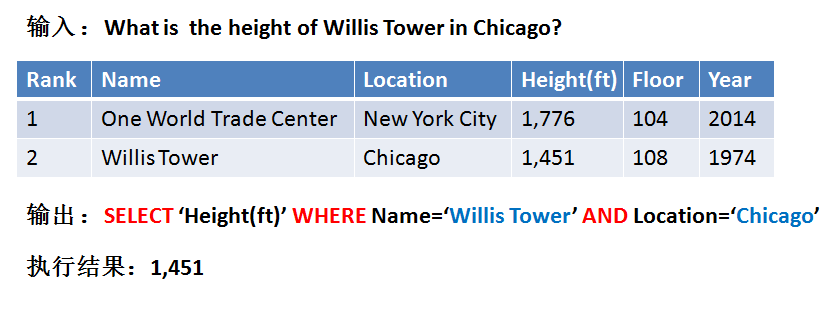
\includegraphics[width=15cm]{example/nl2sql.png}
    \bicaption[NL2SQL的典型示例]
      {NL2SQL的一个典型示例}
      {An Example Of NL2SQL}
    \label{fig:nl2sqlexample}
  \end{figure}

在图\ref{fig:nl2sqlexample}中,$w$代表自然语言问题“What is  the height of Willis Tower in Chicago?”,其中$w_0,w_1,w_2,...$分别代表单词“What”、“is”、“the”等。
$c$代表数据库表的模式“Name Location Height(ft) Floor Year”,其中$c_0,c_1,c_2,...$分别代表单词“Name”、“Location”、“Height(ft)”等。
总输入$x$代表由$w$和$c$组成的集合。
模型的输出$y$在该示例中对应的SQL查询语句为“SELECT ‘Height(ft)’ WHERE Name=‘Willis Tower’ AND Location=‘Chicago’”,其在数据库中执行的结果$r$为1451。

基于深度强化学习的NL2SQL生成的关键问题在于如何去理解自然语言语句的意图并在一次交互的状态下将意图映射到SQL查询语句上,
即在知道数据库表模式$c$的状态下,将用户输入的自然语言问题$w$转换为一条SQL查询语句$y$并得到数据库执行结果$r$。

% 图\ref{fig:nl2sqlexample}为WikiSQL数据集[!!引用!!]中的一个样例。
% WikiSQL数据集是纯自然语言生成SQL查询语句的第一个数据集。
% 其中包含80654组自然语言问句及其对应的SQL查询语句,涵盖24241张从Wikipedia中获取的数据表。
% 从图中可以看到,NL2SQL任务的输入实际包括两部分:自然语言问题以及一个简单的数据表schema(schema代表数据表及表中的列)。

% WikiSQL数据集中SQL查询语句具有一定的约束条件,必须符合如下模板:

% \begin{table}[!hpb]
%     \centering
%     \bicaption[指向一个表格的表目录索引]
%       {SQL查询语句模板}
%       {A Table}
%     \label{nli:sqlmb}
%     \begin{tabular}{@{}llr@{}} \toprule
%       % \multicolumn{2}{c}{Item} \\ \cmidrule(r){1-2}
%     %   节点类型 & 对应的SQL组件\\\midrule
%     \emph{SELECT   agg   selcol   WHERE   col   op   val   (AND   col   op   val)*}\\\bottomrule
  
%       % Animal & Description & Price (\$)\\ \midrule
%       % Gnat & per gram & 13.65 \\
%       % & each & 0.01 \\
%       % Gnu & stuffed & 92.50 \\
%       % Emu & stuffed & 33.33 \\
%       % Armadillo & frozen & 8.99 \\ \bottomrule
%     \end{tabular}
%   \end{table}

%   在\ref{nli:sqlmb}中,\emph{selcol}代表表中的列名,\emph{agg}代表聚合操作(例如:COUNT,SUM或空),
%   \emph{WHERE}后面为由一系列过滤调教构成的子句,每个\emph{op}代表一个过滤操作(例如:“=”),\emph{val}代表出现在自然语言问句中的过滤值。
%   值得注意的是,尽管模板中的过滤条件服从标准的线性顺序,但由于存在\emph{AND}符号,所以过滤条件的先后顺序是无关紧要的。

  

\section{研究现状与相关技术}
\subsection{研究现状}

NL2SQL(Nature Language To SQL Statement)任务可以看作是一种语义解析的任务。
在以前,大多数的研究者提出的语义解析器都依赖弱监督信号,即以SQL查询语句在数据库中的执行结果来构造训练数据,如\cite{goldman2017weakly}。
他们希望能通过训练解析器来生成出SQL语句的基本逻辑形式。
然而,由于SQL语句的逻辑形式往往由人工定义,构造出的训练数据集往往非常小。
同时歧义问题(不同逻辑形式的语句可能产生相同的执行结果,并且无法区分哪种形式是正确结果并作为监督信号)使得设计出来的解析器的性能非常有限。
在2017年,\cite{zhong2017seq2sql}的作者发布了一个由带注释的自然语言查询、SQL查询语句和对应的数据库模式构成的大型数据集WikiSQL。
尽管与之前的SQL生成领域的ATIS和GeoQuery数据集相比,WikiSQL数据集覆盖的SQL语法较少,但是它的优势在于数据集很大并且在自然语言问题的表示和数据库模式和内容上有着非常高的多样性。
这也意味着神经网络和深度学习技术可以更好地应用在NL2SQL这个领域上。

近几年来,已经有大量的研究者在NL2SQL这个领域进行研究并在WikiSQL数据集上进行实验与验证,其中包括\cite{zhong2017seq2sql,dong2016language,xu2017sqlnet,yu2018typesql,wang2018pointing,huang2018natural,wang2018execution}等。
目前主要的研究思路有两种,一种是用基于序列到序列的神经“机器翻译”系统\cite{zhong2017seq2sql,dong2016language},另一种是将SQL查询划分为多个部分并使用不同的模块进行生成\cite{xu2017sqlnet,yu2018typesql}。
第一种方案的挑战在于可能会有多种语义一致的逻辑形式对应于同一个查询结果。
例如\cite{zhong2017seq2sql}中所提到的,由不分先后顺序的过滤条件构成的SQL语句的执行结果却是一致的,而序列到序列的模型往往需要一种标准格式才能训练。
为了解决这个问题,作者使用了强化学习来对解析器的所有正确预测进行奖励。
第二种方案不使用序列到序列模型,而是使用序列到集合的模型先去预测数据表中的哪些列名应该出现在最后的SQL语句中,再在这些列名的基础上分别预测剩余的部分。
这种方法可以有效避免过滤条件的顺序问题,但是也会使得模型丢失很多输入序列的内部依赖信息。
本文总结分析了两种研究思路的优劣,提出了一种新的基于序列到动作的解析器模型。

\subsection{深度学习系统}

% \textbf{深度学习简介}

从网络搜索到社交网络的内容分发,从新闻推荐到电商网站的“猜你喜欢”,机器学习技术已经被广泛应用于我们生活的方方面面,它正在不断地改变和重塑着人类的社会生活。
随着数据的不断涌现,算法的不断改进以及计算能力的不断提升,诸如图片中的目标识别、语音到文字的转换等极具挑战的问题也正在一项项被攻破。
其中最为前卫和火热的技术就是深度学习技术。

深度学习是机器学习的部分内容,其主要为更抽象和高级的数据进行建模和表达。
它具有更强大的能力和灵活性,可以将大千世界表示为嵌套的层次概念体系。
越来越多的智能系统正在从基于规则的系统逐步转向深度学习系统上,如图\ref{fig:DLS}。

\begin{figure}[!htp]
  \centering
  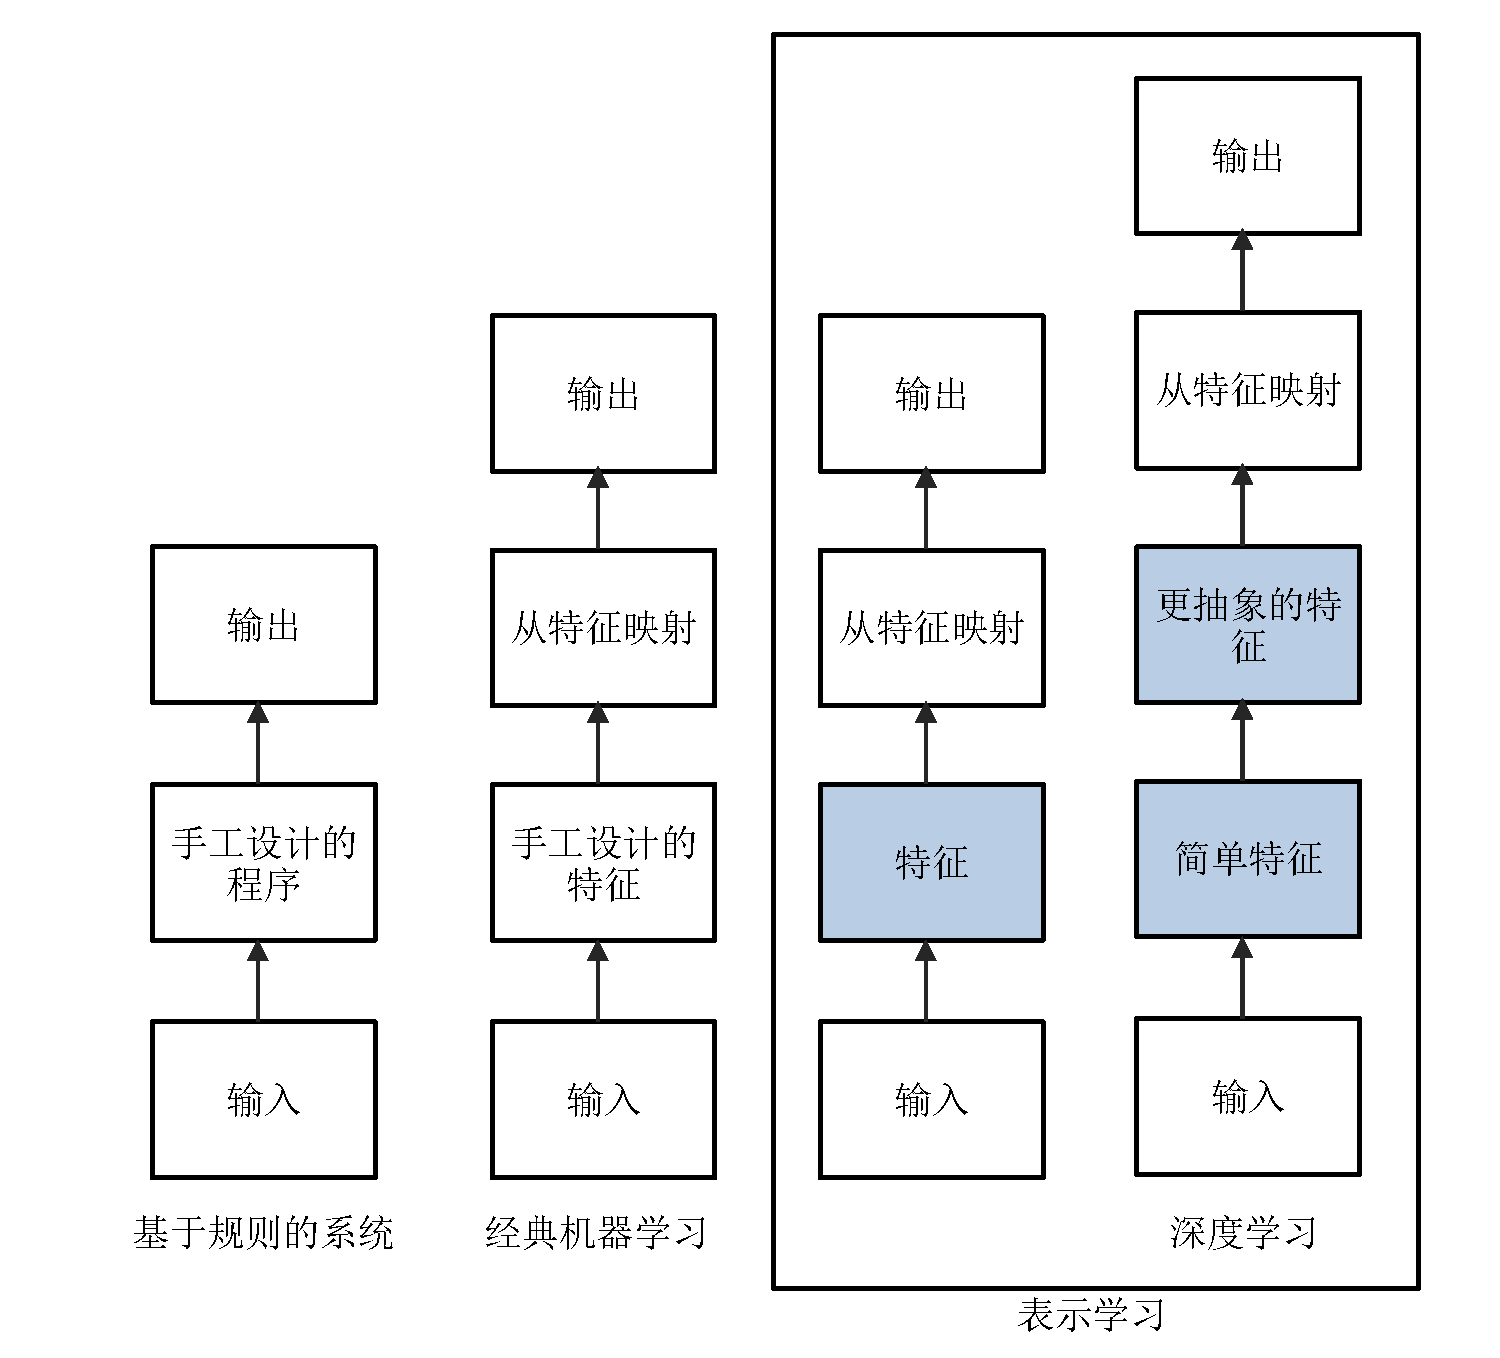
\includegraphics[width=10cm]{example/DLS.pdf}
  \bicaption[智能系统的演变]
    {智能系统的演变\cite{goodfellow2016deep}}
    {The Evolution Of Intelligent Systems}
  \label{fig:DLS}
\end{figure}

接下来,本文将对深度学习的一些基本概念和方法进行介绍,
包括神经网络、反向传播机制、循环神经网络(RNN)、长短期记忆网络(LSTM)、双向循环神经网络(Bi-RNN)和注意力机制(Attention)。

\subsection{神经网络}
% \textbf{神经网络}

\begin{figure}[!htp]
  \centering
  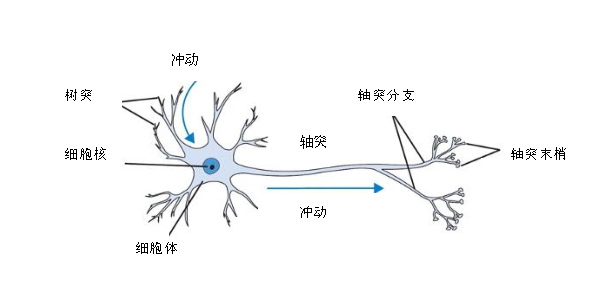
\includegraphics[width=10cm]{example/BNN.pdf}
  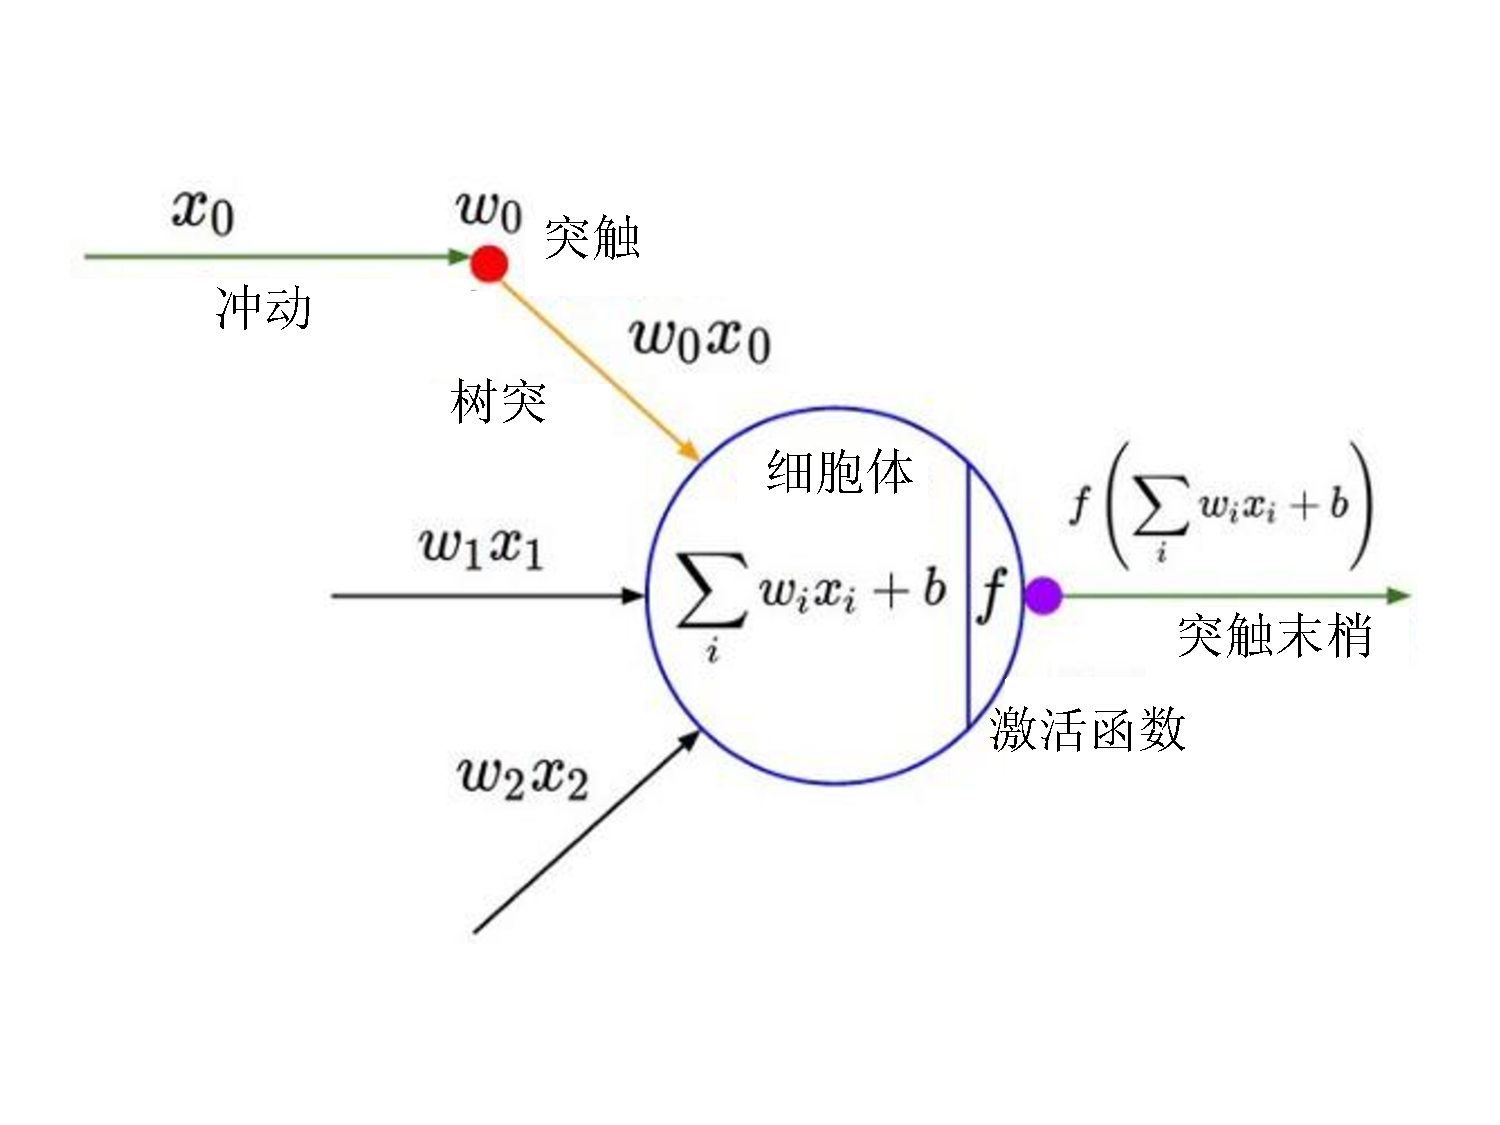
\includegraphics[width=10cm]{example/NNMM.pdf}
  \bicaption[生物神经元及其数学抽象]
    {生物神经元及其数学抽象\cite{goodfellow2016deep}}
    {Biological Neurons And Mathematical Representation}
  \label{fig:BNNandNNMM}
\end{figure}

神经网络(Neural Network)是深度学习的基础,它是一种计算模型,其灵感来源于人脑的生物神经网络处理信息的方式,如图\ref{fig:BNNandNNMM}上。
我们知道大脑的基本计算单元是神经元,人类的神经系统中大约有860亿个神经元以及与之相连的$10^{10}$至$10^{15}$个突触。
计算机科学家将神经元的工作原理抽象成为数学的表达形式,如图\ref{fig:BNNandNNMM}下。

% \begin{figure}[!htp]
%   \centering
%   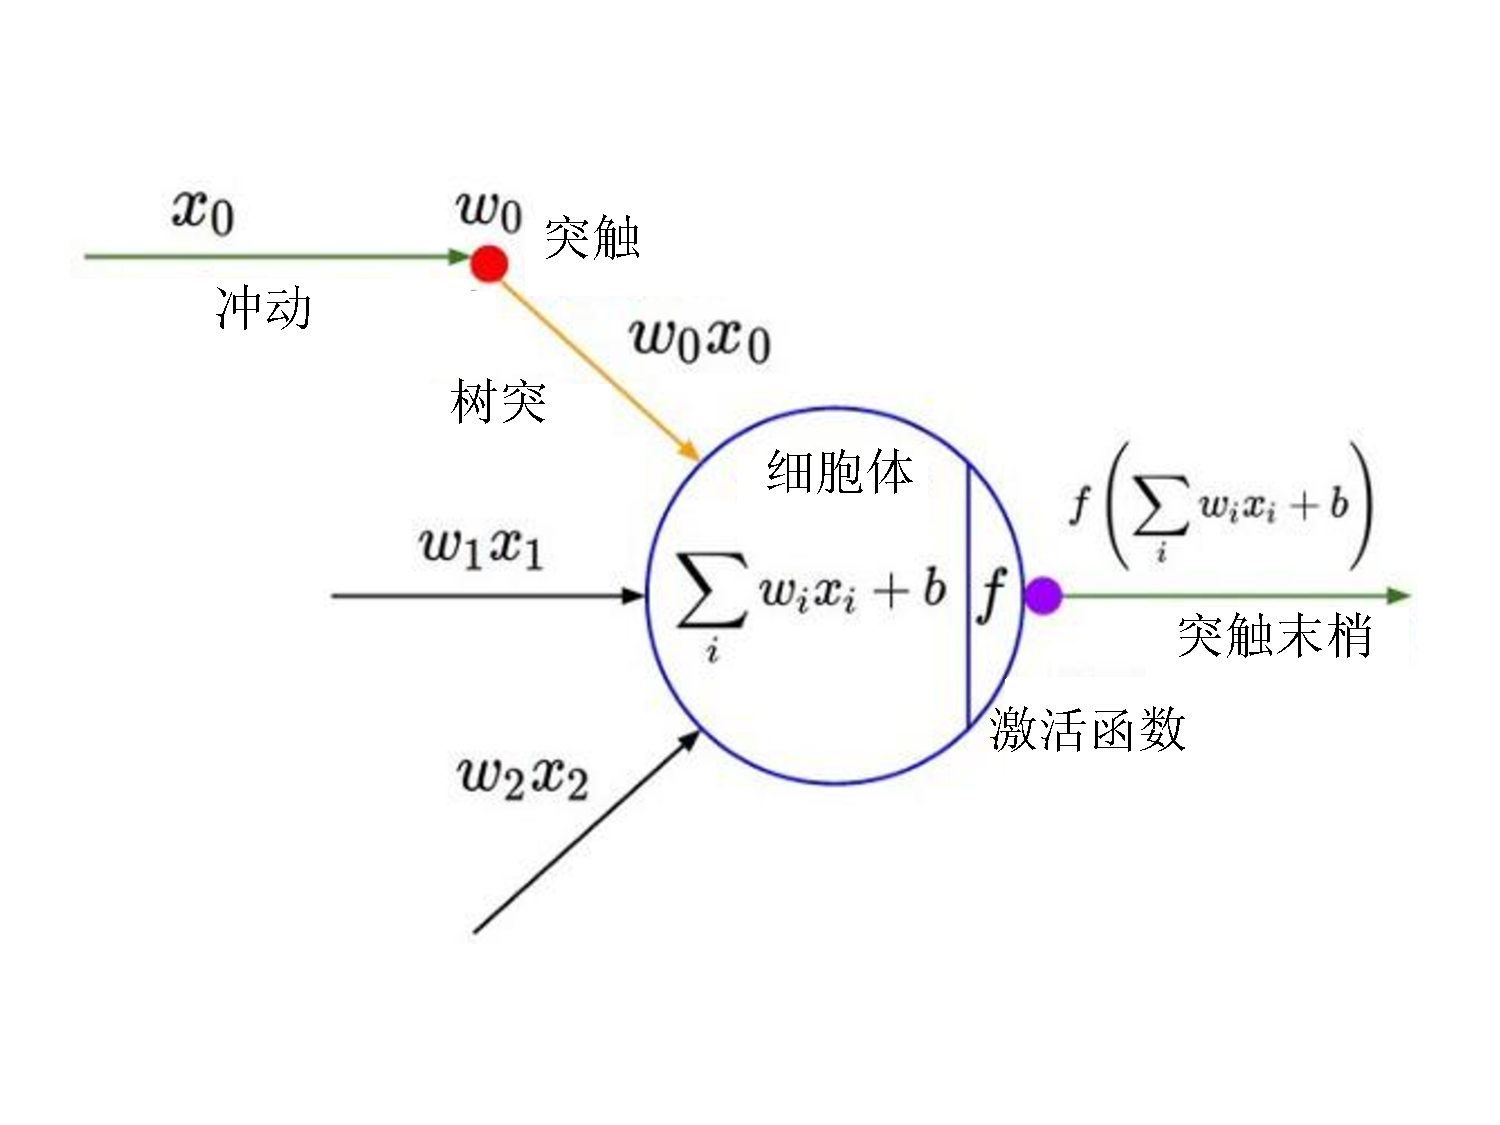
\includegraphics[width=8cm]{example/NNMM.pdf}
%   \bicaption[这里将出现在插图索引中]
%     {神经元的数学抽象}
%     {English caption}
%   \label{fig:NNMM}
% \end{figure}

简单来说,神经网络中的基本计算单元是神经元(Cell),也被叫做节点(Node)或单元(Unit)。
它接收来自其他的节点或者外部数据源的输入,经过计算之后得到输出。
每个输入$x_i$都会有一个对应的权重$w_i$,通过$\sum_i w_ix_i$计算加权和之后再加上一个偏置$b$(bias)。
最后通过激活函数$f$得到输出$f(\sum_i w_ix_i +b)$。

其中,激活函数$f$是非线性函数,通过引入非线性的激活函数来模拟当细胞接受到的信号总和超过某个阈值时产生激活。
我们常常会使用三种激活函数,分别为$softmax$、$tanh$和$ReLU$,如公式\ref{enl2sql:afeq}和图\ref{fig:af}(图中从左到右分别为$softmax$、$tanh$和$ReLU$函数)所示。

\begin{gather}
  \label{enl2sql:afeq}
  sigmoid(x) = \frac{1}{1 + e^{-x}}\\
  tanh(x) = \frac{2}{1 + e^{-2x}} - 1\\
  ReLU(x) = \max(0,x)
\end{gather}

\begin{figure}[!htp]
  \centering
  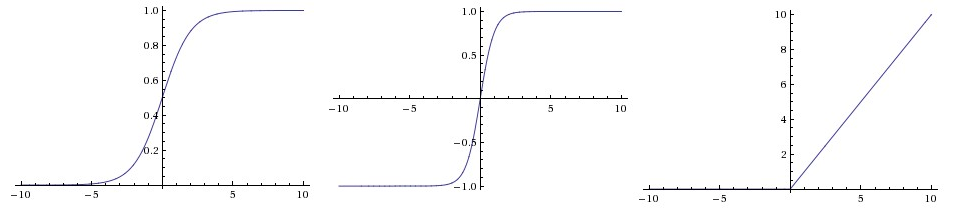
\includegraphics[width=14cm]{example/af.png}
  \bicaption[激活函数]
    {激活函数}
    {Activation Function}
  \label{fig:af}
\end{figure}

为了处理更大的数据量,我们一般将许多的神经元组合在一起并分为不同的层(layer),从而构成神经网络的基础架构,如图\ref{fig:NNA}所示。
其中主要包含三种层:

\begin{itemize}
  \item 输入层(input layer):输入层接收由外部输入的数据并传递给下一层,不进行任何的计算。
  \item 隐藏层(hidden layer):隐藏层进行数据处理和计算,将计算结果传递给下一层。在网络中可以存在多个隐藏层,其节点个数也可能不一致。
  \item 输出层(output layer):输出层往往会将结果映射到所需的输出格式上,例如采用$softmax$函数进行多分类。
\end{itemize}

\begin{figure}[!htp]
  \centering
  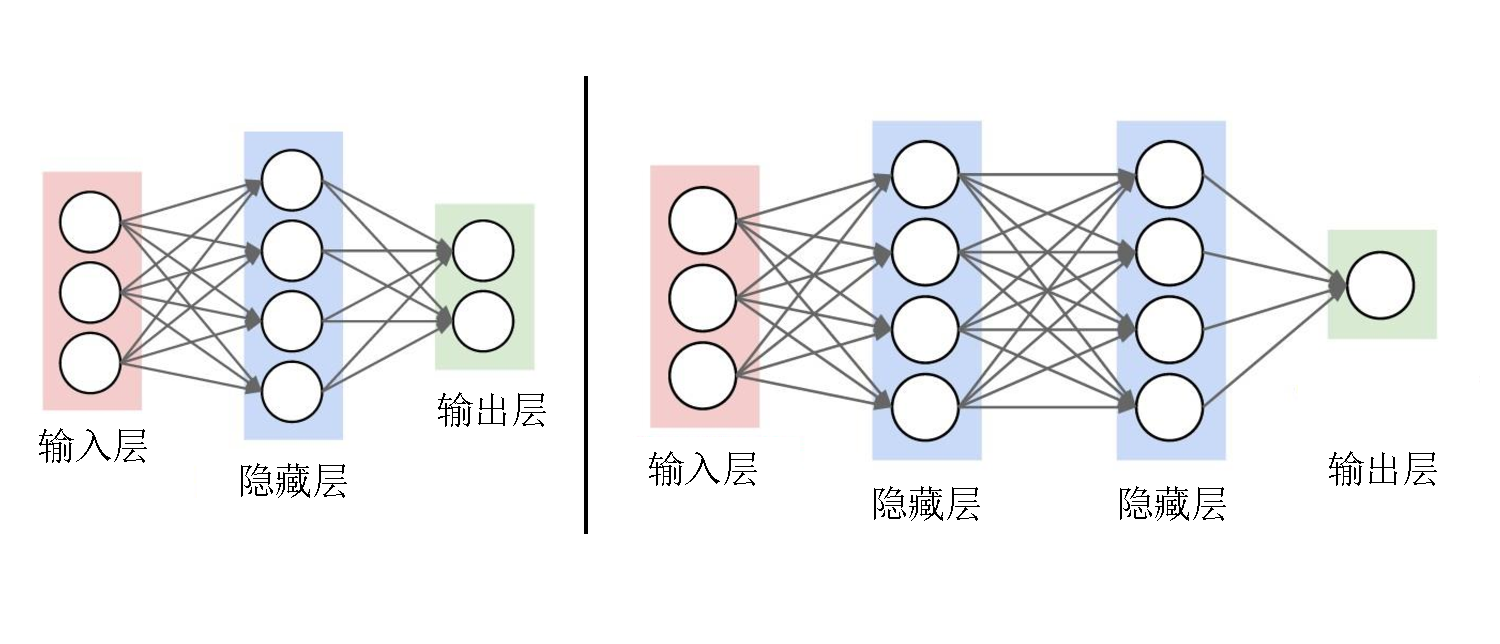
\includegraphics[width=13cm]{example/NNA.pdf}
  \bicaption[神经网络的基础架构]
    {神经网络的基础架构}
    {The Basic Infrastructure of Neural Network}
  \label{fig:NNA}
\end{figure}

\subsection{反向传播机制}
% \textbf{反向传播机制}

反向传播(Backward Propagation)机制\cite{rumelhart1986learning}是训练神经网络的几种方式之一,使用它可以利用训练数据来进行监督学习。
简单来说,反向传播就是“从错误中学习”,每当计算结果与正确结果不一致时,反向传播机制可以有效地纠正神经网络。
从图\ref{fig:BP}可以看出,首先经过前向传播得到模型的输出与正确结果之间的总误差$E_{total}$,然后使用链式法则将误差向后传播并得到所有向量和权重的更新梯度。

\begin{figure}[!htp]
  \centering
  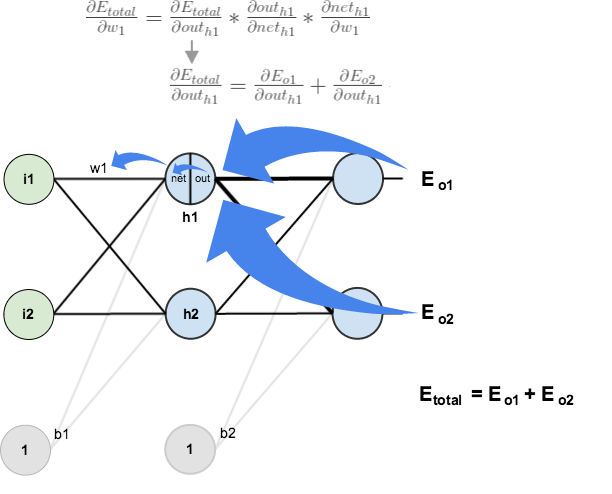
\includegraphics[width=10cm]{example/BP.png}
  \bicaption[反向传播机制]
    {反向传播机制}
    {Back Propagation Mechanism}
  \label{fig:BP}
\end{figure}

\subsection{循环神经网络}
% \textbf{循环神经网络(RNN)}

深度学习领域有两个非常经典和实用的网络,一个是卷积神经网络(CNN),另一个则是循环神经网络(RNN)\cite{goodfellow2016deep}。
与CNN不同的是,RNN是一种序列模型,例如把一个英文自然语言句子作为输入时,RNN会按照单词在句子中的顺序单独输入给网络,每次的输出都取决于之前网络计算的结果。
经典的循环神经网络如图\ref{fig:RNN}所示。
其中:
\begin{itemize}
  \item $x_t$代表$t$时刻的输入。例如,$x_0$表示输入句子中第一个单词的One-hot编码向量。
  \item $s_t$代表$t$时刻隐藏层的状态,是网络的“记忆”。$s_t$通过上一时刻的隐藏状态和当前时刻的输入经过$s_t = f(Ux_t + Ws_{t-1})$计算得到。其中$f$为激活函数,$s_{-1}$初始化为零。
  \item $o_t$代表$t$时刻的输出。例如,我们想要预测出句子中下一个单词是什么,则$o_t$就是一个概率向量$o_t = softmax(Vs_t)$来表示词汇表中每个单词出现的概率。
\end{itemize}

\begin{figure}[!htp]
  \centering
  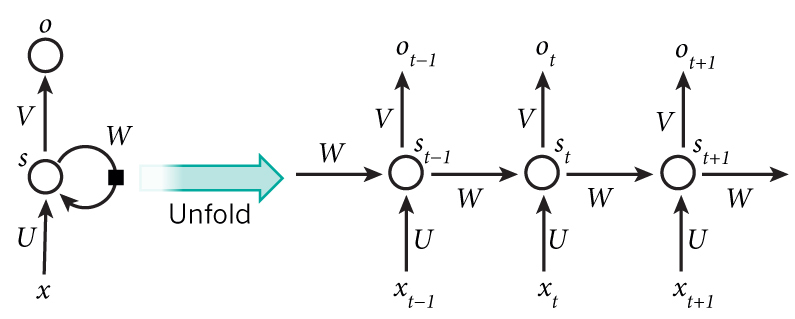
\includegraphics[width=11cm]{example/RNN.jpg}
  \bicaption[循环神经网络]
    {循环神经网络}
    {Recurrent Neural Network}
  \label{fig:RNN}
\end{figure}

\subsection{长短期记忆网络}
% \textbf{长短期记忆网络(LSTM)}

经典的循环神经网络有一个明显的缺点,就是当时刻变得很长时,网络无法利用到很早之前的上下文信息。
为了解决这个问题,Hochreiter和Schmidhuber发明了一种能够进行长期“记忆”的网络,长短期记忆网络(LSTM)\cite{goodfellow2016deep}。
如图\ref{fig:LSTM}所示(黄色矩形表示神经网络层;粉色圆形表示运算操作,如加、减、乘、除;黑色单箭头表示向量的传输;合成箭头表示向量的连接;分箭头表示向量的复制),LSTM的结构与RNN保持一致,只是在隐藏层内部做了很多的“记忆”操作,包括:

\begin{itemize}
   \item 遗忘门(forget gate),目的为从细胞状态中丢弃信息,表示为$f_t$。
   \item 更新门(update gate),目的为让新的信息加入到细胞状态中,表示为$i_t$、$\widetilde{C}_t$和$C_t$。
   \item 输出门(output gate),目的为确定输出的值,表示为$o_t$和$h_t$。
\end{itemize}

\begin{figure}[!htp]
  \centering
  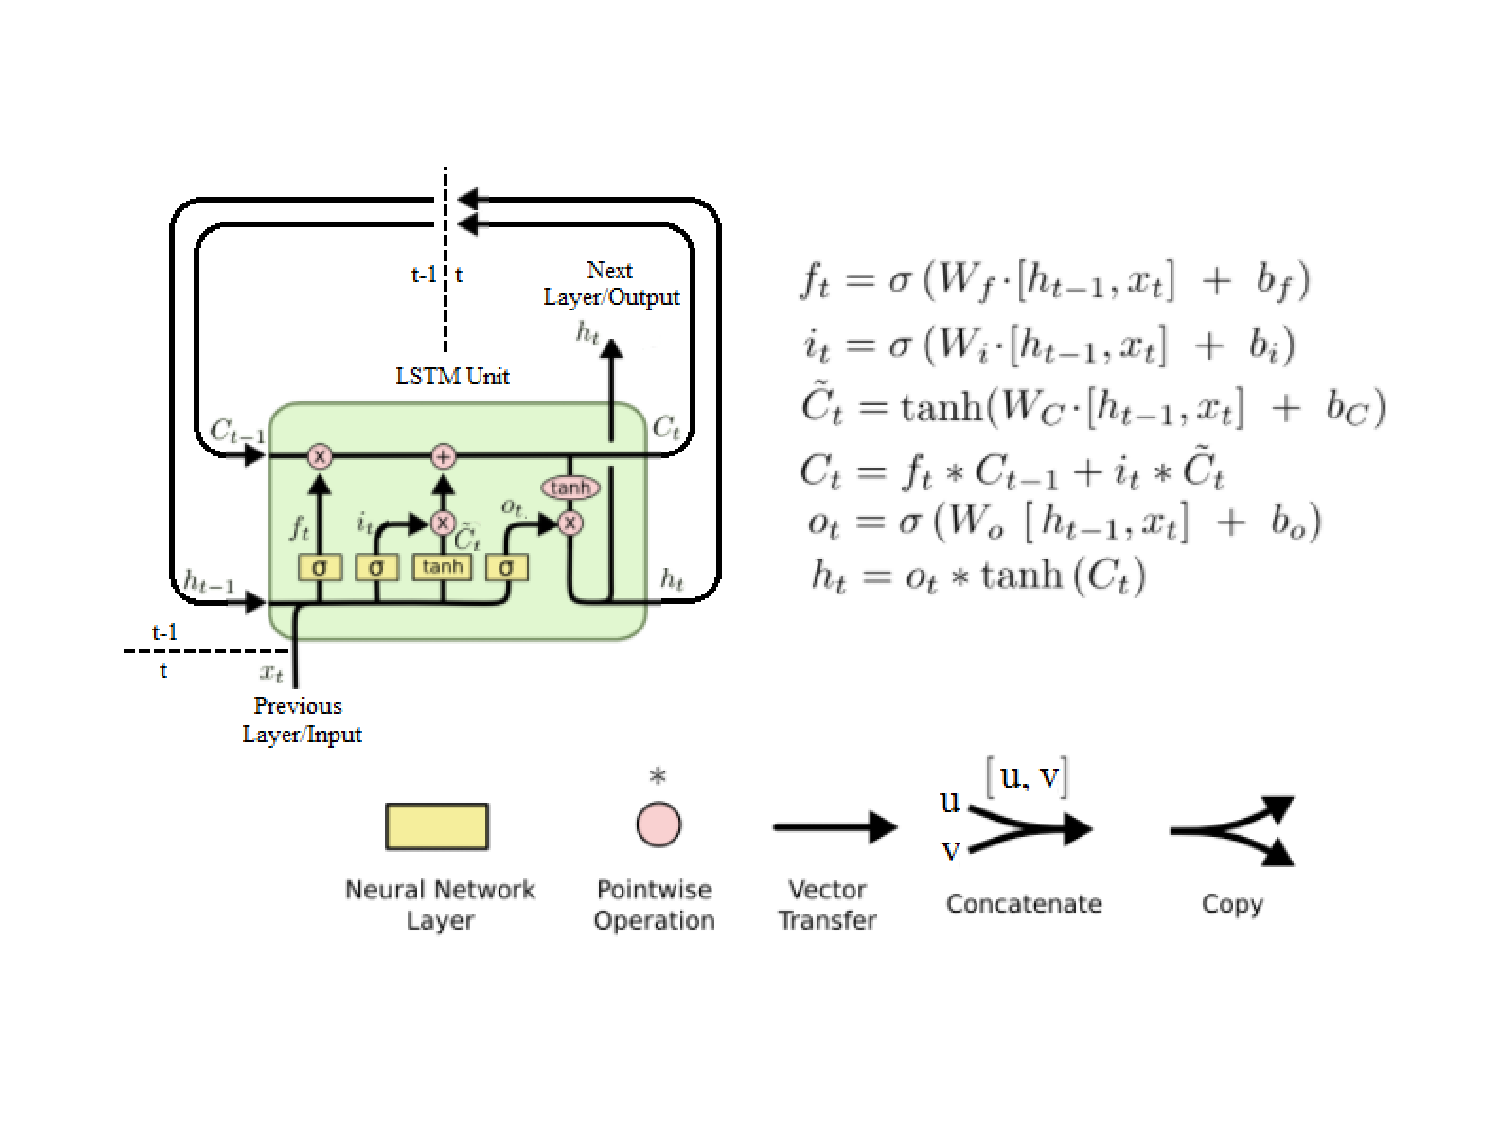
\includegraphics[width=13cm]{example/LSTM.pdf}
  \bicaption[长短期记忆网络]
    {长短期记忆网络(LSTM)}
    {Long Short-Term Memory}
  \label{fig:LSTM}
\end{figure}

\subsection{双向循环神经网络}
% \textbf{双向循环神经网络}

包括RNN、LSTM、GRU在内的很多网络都有一个共同的缺陷就是网络只会对之前时刻的信息进行学习。
而实际上,在很多场景下我们需要从未来时刻的信息中学习。
双向循环神经网络(Bi-RNN)及其变种的出现就是为了解决这个问题。

Bi-RNN的结构如图\ref{fig:BiRNN}所示,其中的重复模块可以是经典的RNN、LSTM或GRU。
网络可以分为两个部分的连接,先是从前向后执行学习到以前的信息,再由后向前在未来的表示中学习。

\begin{figure}[!htp]
  \centering
  \includegraphics[width=11cm]{example/BiRNN.png}
  \bicaption[双向循环神经网络]
    {双向循环神经网络(Bi-RNN)}
    {Bidirectional Recurrent Neural Network}
  \label{fig:BiRNN}
\end{figure}

\subsection{注意力机制}
% \textbf{注意力机制(Attention)}

传统的序列到序列的网络结构将原句子编码为固定长度的向量再输入给解码器,这将导致大量的信息丢失。
为了解决这个问题,谷歌提出了名为注意力机制(Attention)的解决方案。

\begin{figure}[htbp]
  \centering
  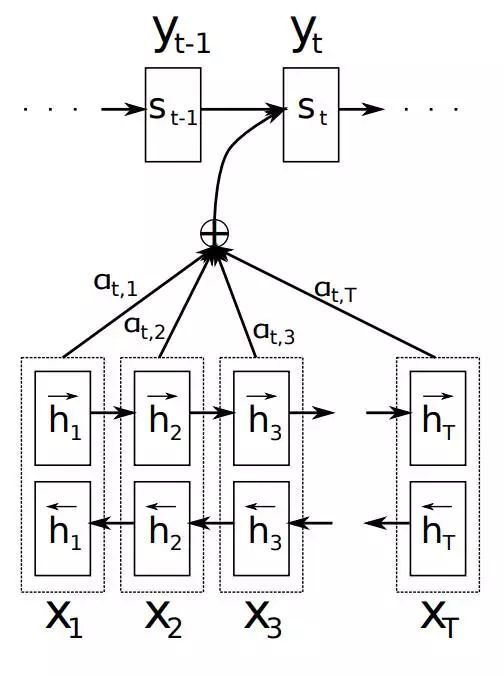
\includegraphics[width=5cm]{example/attention1.jpg}
  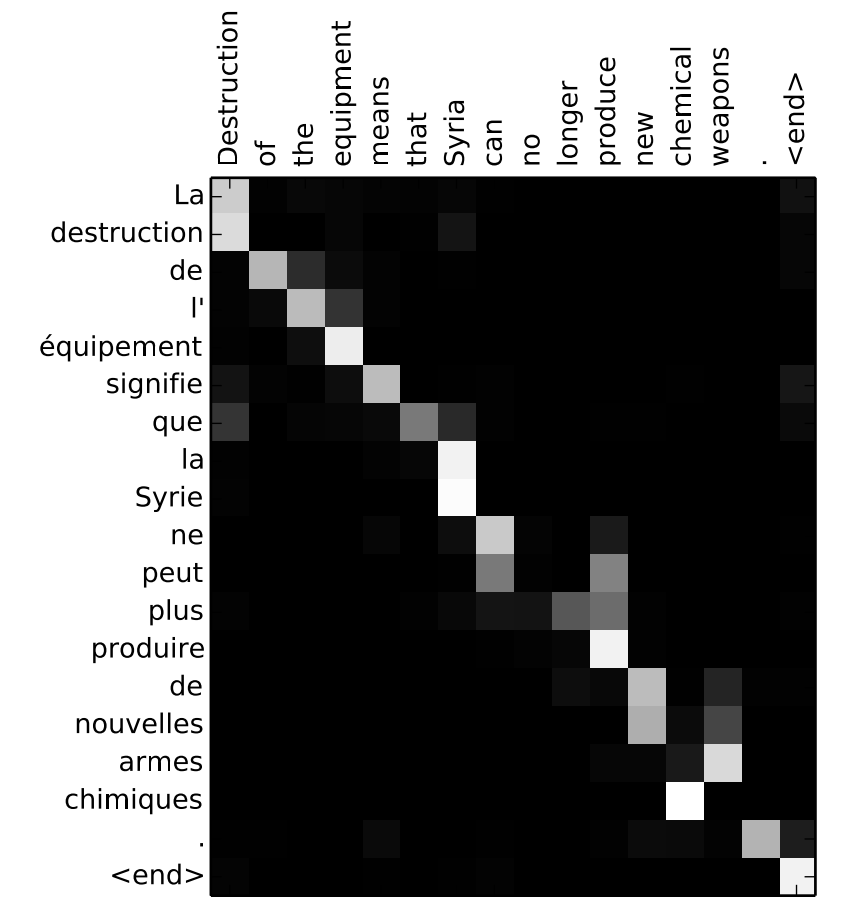
\includegraphics[width=7cm]{example/attention2.png}
  % \subfigure[注意力机制1]{
  %   \includegraphics[width=5.5cm]{BiRNN.png}
  %   %\caption{fig1}
  % }
  % \quad
  % \subfigure[注意力机制2]{
  %   \includegraphics[width=5.5cm]{BiRNN.png}
  %   %\caption{fig1}
  % }
  % \subfigure[注意力机制1] %第一张子图
  % {
  %   \begin{minipage}{7cm}
  %   \centering          %子图居中
  %   \includegraphics[scale=0.1]{BiRNN.png}   %以pic.jpg的0.5倍大小输出
  %   \end{minipage}
  % } 
  % \subfigure[注意力机制2] %第二张子图
  % {
  %   \begin{minipage}{7cm}
  %   \centering      %子图居中
  %   \includegraphics[scale=0.1]{BiRNN.png}   %以pic.jpg的0.5倍大小输出
  %   \end{minipage}
  \bicaption[注意力机制原理及可视化]
    {注意力机制原理及可视化}
    {Attention Mechanism And Visualization}
\label{fig:attention}
\end{figure}

图\ref{fig:attention}中左侧为注意力机制原理。
其中,$y$表示在翻译过程中解码器生成的单词,$x$表示输入的原句子。
每个解码器输出的$y_t$现在不单是取决于网络上一时刻的状态,而是取决于它和输入的加权组合。
$a$为权重,表示输出时应当考虑多少输入状态。
例如,若$a_{3,2}$是一个很大的数字,表示网络认为输出的第三个单词、与输入的第二个单词的关联度很高。
图\ref{fig:attention}中右侧为注意力机制的可视化展示,使得我们能够解释模型的一些内部原理。
例如,将法语翻译为英语时网络将“la Syrie”翻译为“Syria”,可视化结果表明模型在此刻将两个单词关联到一个单词上而不是一一对应。


% \subsection{强化学习}
\subsection{强化学习}
% \textbf{强化学习}

机器学习可以分为三种学习类型,分别为非监督学习、监督学习和强化学习。
强化学习是主要依靠智能体在环境(environment)中不断地试错并采取一系列的行为(action)从而累积得到最大的奖励(reward)的过程,
其范式(如图\ref{fig:RL}所示)类似于人类学习知识的过程。
一般来说,强化学习由智能体和环境两个部件组成,主要有以下四个要素:状态(state)、动作(action)、智能体(agent)和奖励(reward)。
以小孩学习走路为例,小孩是智能体,他通过采取动作(即行走)来操纵环境(行走的表面),并且从一个状态转变到另一个状态(即他走的每一步),当他完成任务的子任务(即走了几步)时,孩子得到奖励(给巧克力吃),并且当他不能走路时,就不会给巧克力。

从算法的角度,强化学习可以分为三类:
\begin{itemize}
  \item 基于策略(Policy based)的强化学习。其目标为找到最优的策略。
  \item 基于价值(Value based)的强化学习。其目标为奖励综合的最大化。
  \item 基于动作(Action based)的强化学习。其目标为最优动作的执行。
\end{itemize}
\begin{figure}[!htp]
  \centering
  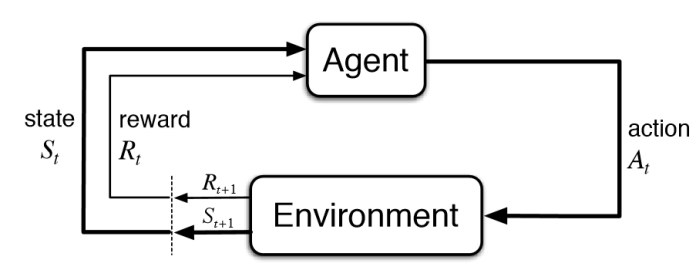
\includegraphics[width=11cm]{example/RL.jpg}
  \bicaption[强化学习范式]
    {强化学习范式}
    {The Paradigm of Reinforcement Learning}
  \label{fig:RL}
\end{figure}

% \textbf{深度强化学习}

% \subsection{语义解析}

\section{解决方案}

介绍完本章的研究问题、研究现状和相关技术之后,我们将在本节中给出基于深度强化学习的NL2SQL生成的解决方案。

\subsection{技术方案}
\begin{figure}[!htp]
  \centering
  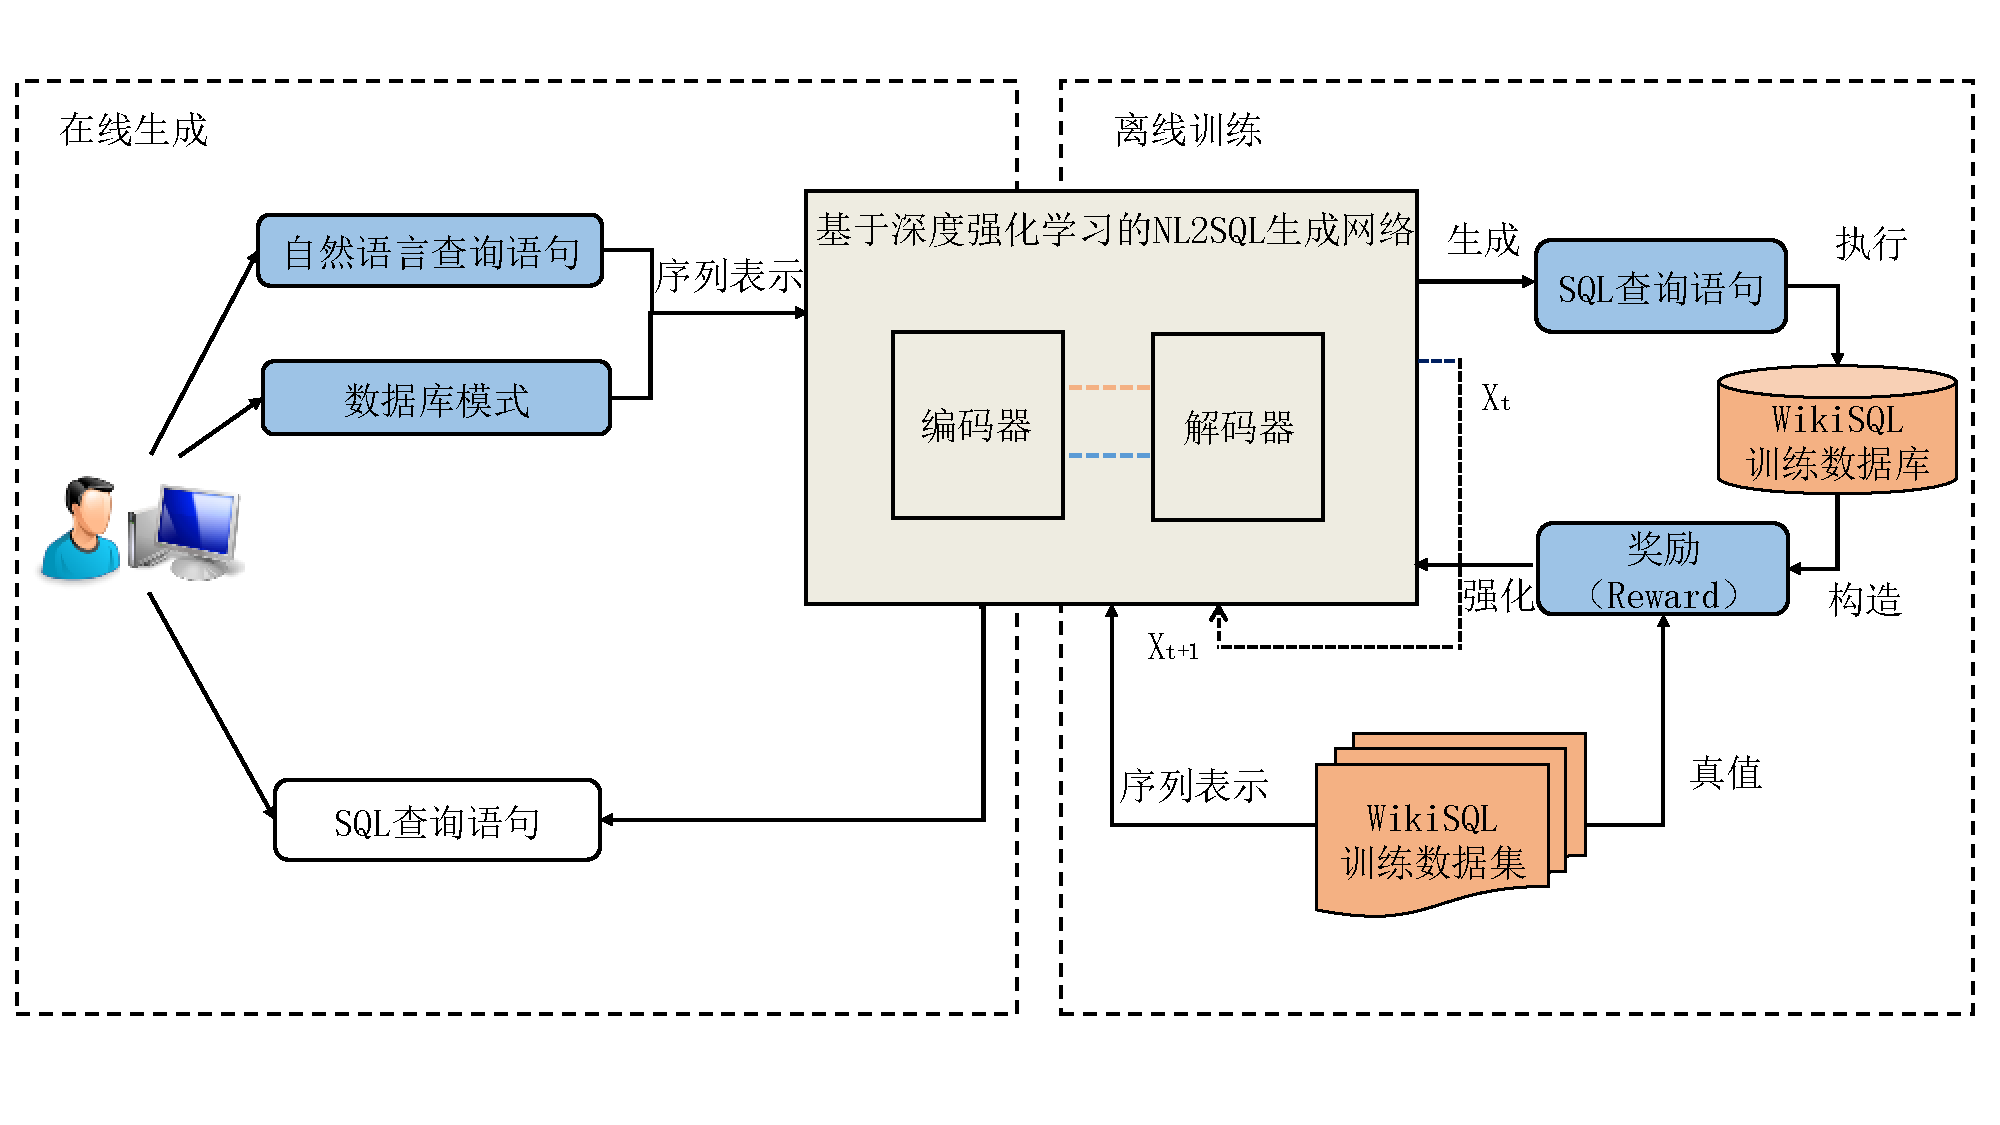
\includegraphics[width=15cm]{example/nl2sqlapproach.pdf}
  \bicaption[基于深度强化学习的NL2SQL生成的技术方案]
    {基于深度强化学习的NL2SQL生成的技术方案}
    {The Approach of NL2SQL With Deep Reinforcement Learning}
  \label{fig:nl2sqlapproach}
\end{figure}

基于深度强化学习的NL2SQL生成的技术方案如图\ref{fig:nl2sqlapproach}所示,包含离线训练和在线生成两部分。

在离线训练中,我们从WikiSQL数据集中获取自然语言查询语句及其对应的数据库模式数据并进行序列的向量编码表示(Embedding),
基于深度强化学习的NL2SQL生成网络使用这些序列表示作为输入并输出一条SQL查询语句,
将该语句导入数据库进行执行后得到执行结果并交由奖励函数进行计算,得到奖励后对原网络进行强化。
需要说明的是,在后文中,我们把基于深度强化学习的NL2SQL生成网络命名为增强解析器,它由编码器(Encoder)和解码器(Decoder)组成,是基于时间序列的模型。

在在线生成中,用户可以输入自然语言查询语句以及其对应的数据库模式,系统将对输入序列进行向量编码表示,
基于深度强化学习的NL2SQL生成网络将生成并返回给用户一条SQL查询语句。

接下来,本文将对技术方案中最重要的增强解析器模型(即基于深度强化学习的NL2SQL生成网络)进行介绍。

\subsection{增强解析器模型}
\label{enl2sql:zqjxqmx}
首先,针对输入$x$来生成结构化的输出$y$的过程可以被分解成为一系列的语义解析决策的过程。
我们参考强化学习的基本范式,将增强解析器模型的基本过程定义为:

\begin{itemize}
  \item 解析器(agent)从初始状态启动并不断根据学习的策略采取不同的动作(action)。每个动作都会将解析器从一个状态(state)转移为另一个状态,直到解析器到达它的最终状态并停止。在解析器的最终状态下,我们可以得到输出$y$。
\end{itemize}

在这里,我们采取一种概率的方法来对整个策略(policy)进行建模。
我们通过对输入$x$产生的所有动作(action)和解码器产生的历史行为建模得到一个概率分布。
而整个增量语义解析器的训练目标就转换为了如何去优化一个参数化的策略的问题,如公式公式\ref{enl2sql:eq1}所示。

% , 其中$\theta$为模型参数。
\begin{equation}
    \label{enl2sql:eq1}
    % Sim \left ( n ,\right v) = \max\left ( Sim_{wup}\left ( n ,\right v) ,\right Sim_{gram}\left ( n ,\right v))
    % Sim(n,v) = \max(Sim_{wup}(n,v),Sim_{gram}(n,v))
    % P_{\theta}(y|x) = P_{\theta}(\boldsymbol{a}|x),   \theta为模型参数
    P_{\theta}(y|x) = P_{\theta}(\boldsymbol{a}|x),  \qquad \theta\text{为模型参数}
\end{equation}

在公式\ref{enl2sql:eq1}中,$\theta$为模型参数,通过执行动作(action)序列$\boldsymbol{a} = \{a_{1},a_{2},...,a_{k}\}$,解析器将被不断引导并从初始状态转换为包含输出$y$的最终状态。
在此,我们需要假设每个输出$y$有且仅有一个对应的动作序列$\boldsymbol{a}$(详见\ref{enl2sql:ndo}节内容)。
行动序列的概率$P_{\theta}(\boldsymbol{a}|x)$可展开为增量策略概率的乘积(公式\ref{enl2sql:eq2}):

\begin{equation}
    \label{enl2sql:eq2}
    % Sim \left ( n ,\right v) = \max\left ( Sim_{wup}\left ( n ,\right v) ,\right Sim_{gram}\left ( n ,\right v))
    % Sim(n,v) = \max(Sim_{wup}(n,v),Sim_{gram}(n,v))
    P_{\theta}(\boldsymbol{a}|x) = \prod^k_{i=1}P_{\theta}(a_{i}|x,a_{<i}),   \qquad |\boldsymbol{a}| = k
\end{equation}

在在线生成期间,我们的模型并非尝试枚举整个输出空间并找到最高的得分$\boldsymbol{a}^{*} = \mathop{\arg\max}_{\boldsymbol{a}} P_{\theta}(\boldsymbol{a}|x)$,
而是在解码器中采用了一种贪心的方法:在每一步都根据策略(policy)来选择得分最高的行动,即$a^{*}_{i} = \mathop{\arg\max}_{a_{i}} P_{\theta}(a_{i}|x,a^{*}_{<i})$。

在后面的几节中,我们将给出增强解析器的状态(state)的定义以及动作(action)清单,还会详细介绍整个基于编码器-解码器神经网络体系结构的增强解析器模型。

% \begin{figure}[!htp]
%   \centering
%   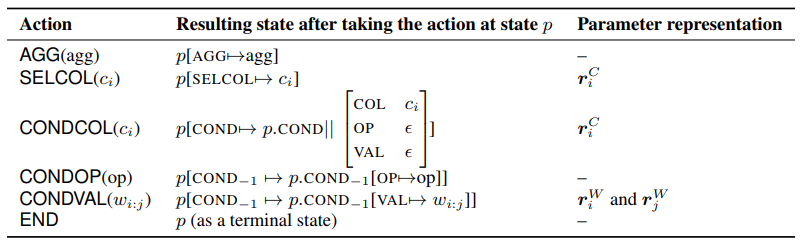
\includegraphics[width=20cm]{example/incsql.png}
%   \bicaption[这里将出现在插图索引中]
%     {中文题图}
%     {English caption}
%   \label{fig:SRR}
% \end{figure}

\subsection{动作序列}
\label{enl2sql:dzxl}

首先,我们给出对应于图\ref{fig:nl2sqlexample}中示例的完全解析之后的结构化表示:
% $\begin{Bmatrix}
%   1 & 2 \\
%   4 & 3 \\
% \end{Bmatrix}$
% \begin{bmatrix}
  
% \end{bmatrix}

$\begin{bmatrix}
  AGG    &  NONE  \\
  SELCOL &  Height(ft) \\
  COND   &   \langle
  % \begin{Bmatrix}
    \begin{bmatrix}
      COL  &  Name \\
      OP   &  =    \\
      VAL  &  “Willis Tower”\\
    \end{bmatrix}
    ,
    \begin{bmatrix}
      COL  &  Location \\
      OP   &  =    \\
      VAL  &  “Chicago”\\
    \end{bmatrix}
    % \end{Bmatrix}
    \rangle
  \end{bmatrix}$

因此,解析器的中间状态就被这样分部表示,其中一些尚未填充的特征值表示为$\epsilon$。
解析器的初始状态$p_{0}$的值为空和空列表,表示为$\begin{bmatrix}
  AGG    &  \epsilon  \\
  SELCOL &  \epsilon \\
  COND   &   \langle \rangle\\
  \end{bmatrix}$。

除此之外,我们还需要定义动作(action)清单。每个动作可以将解析器的状态从一个状态转换为另一个状态,即 $p \rightarrow p_{'}$ 。
我们设$p = \begin{bmatrix}
  AGG    &  agg  \\
  SELCOL &  selcol \\
  COND   &   cond\\
  \end{bmatrix}$,并且在表\ref{enl2sql:dzqd}中给出每个动作执行后的转移状态$p'$。

  \begin{table}[!hpb]
    \centering
    \bicaption[动作清单]
      {动作(action)清单}
      {The Inventory Of Actions }
    \label{enl2sql:dzqd}
    \begin{tabular}{@{}llr@{}} \toprule
      % \multicolumn{2}{c}{Item} \\ \cmidrule(r){1-2}
      \textbf{动作(action)} & \textbf{由状态}$p$\textbf{执行该动作之后的状态} & \textbf{参数表示}\\\midrule
      % 1  & 	Q -> ( SClause ) ( ComplexCondition ) *\\
      AGG($agg$)  &  $p[AGG \mapsto agg]$  & - \\
      SELCOL($c_i$)  &  $p[SELCOL \mapsto c_i]$  & $r^C_i$ \\
      CONDCOL($c_i$)  &  $p[COND \mapsto p.COND||\begin{bmatrix}
        COL    &  c_i  \\
        OP &  \epsilon \\
        VAL   &   \epsilon\\
        \end{bmatrix}]$  &  $r^C_i$\\
      CONDOP(op)  &  $p[COND_{-1} \mapsto p.COND_{-1}[OP \mapsto op]]$  & -\\
      CONDVAL($w_{i:j}$)  &  $p[COND_{-1} \mapsto p.COND_{-1}[VAL \mapsto w_{i:j}]]$  &  $r^W_i and r^W_j$\\
      END  &  $p$(最终状态)  &  -\\\bottomrule
    \end{tabular}
  \end{table}

需要说明的是,在表\ref{enl2sql:dzqd}中,在解码器中所使用的参数表示将在\ref{enl2sql:decoder}节中进行解释;
$p[AGG \mapsto agg]$表示与状态$p$处于同一状态,不过其特征值$AGG$已经被赋值为$agg$;
$||$表示列表展开;$COND_{-1}$表示在列表中的上一个元素;


需要特别解释的是,动作$CONDVAL$会从输入问句$w$中选择所需的文字段$w_{i:j}$。
但这样做会导致一个问题,它将产生大量的动作,其数量级为问题长度的二次方。
因此,我们将动作$CONDVAL$分解为两个连续的子动作,一个去选择起始位置$w_i$,另一个则选择终止位置$w_j$。
在动作序列的最后,我们需要增加一个$END$动作来执行解析过程并使解析器进入结束状态。
举例来说,图\ref{fig:nl2sqlexample}中的例子可以看作是如下的一个动作序列:
\begin{enumerate}
  \item $AGG(NONE)$
  \item $SELCOL(c_3)$
  \item $CONDCOL(c_1)$
  \item $CONDOP(=)$
  \item $CONDVAL(w_{5:6})$
  \item $CONDCOL(c_2)$
  \item $CONDOP(=)$
  \item $CONDVAL(w_{8:8})$
  \item $END$
\end{enumerate}
% ${AGG(NONE),SELCOL(c_3),CONDCOL(c_1),CONDOP(=),CONDVAL(w_{5:6}),CONDCOL(c_2),CONDOP(=),CONDVAL(w_{8:8})}$

需要注意的是该节中的定义是基于所有有效序列都具有AGG  SELCOL  (CONDCOL  CONDOP  CONDVAL)* END形式的假设之上。
这样的假设能够保证我们可以从所有的最终状态输出中提取出完整的逻辑形式出来。
对于其他不同结构的SQL语句来说,我们还需要重新设计动作的清单以及解析器的状态。


\subsection{编码器}
\label{enl2sql:encoder}

\begin{figure}[!htp]
  \centering
  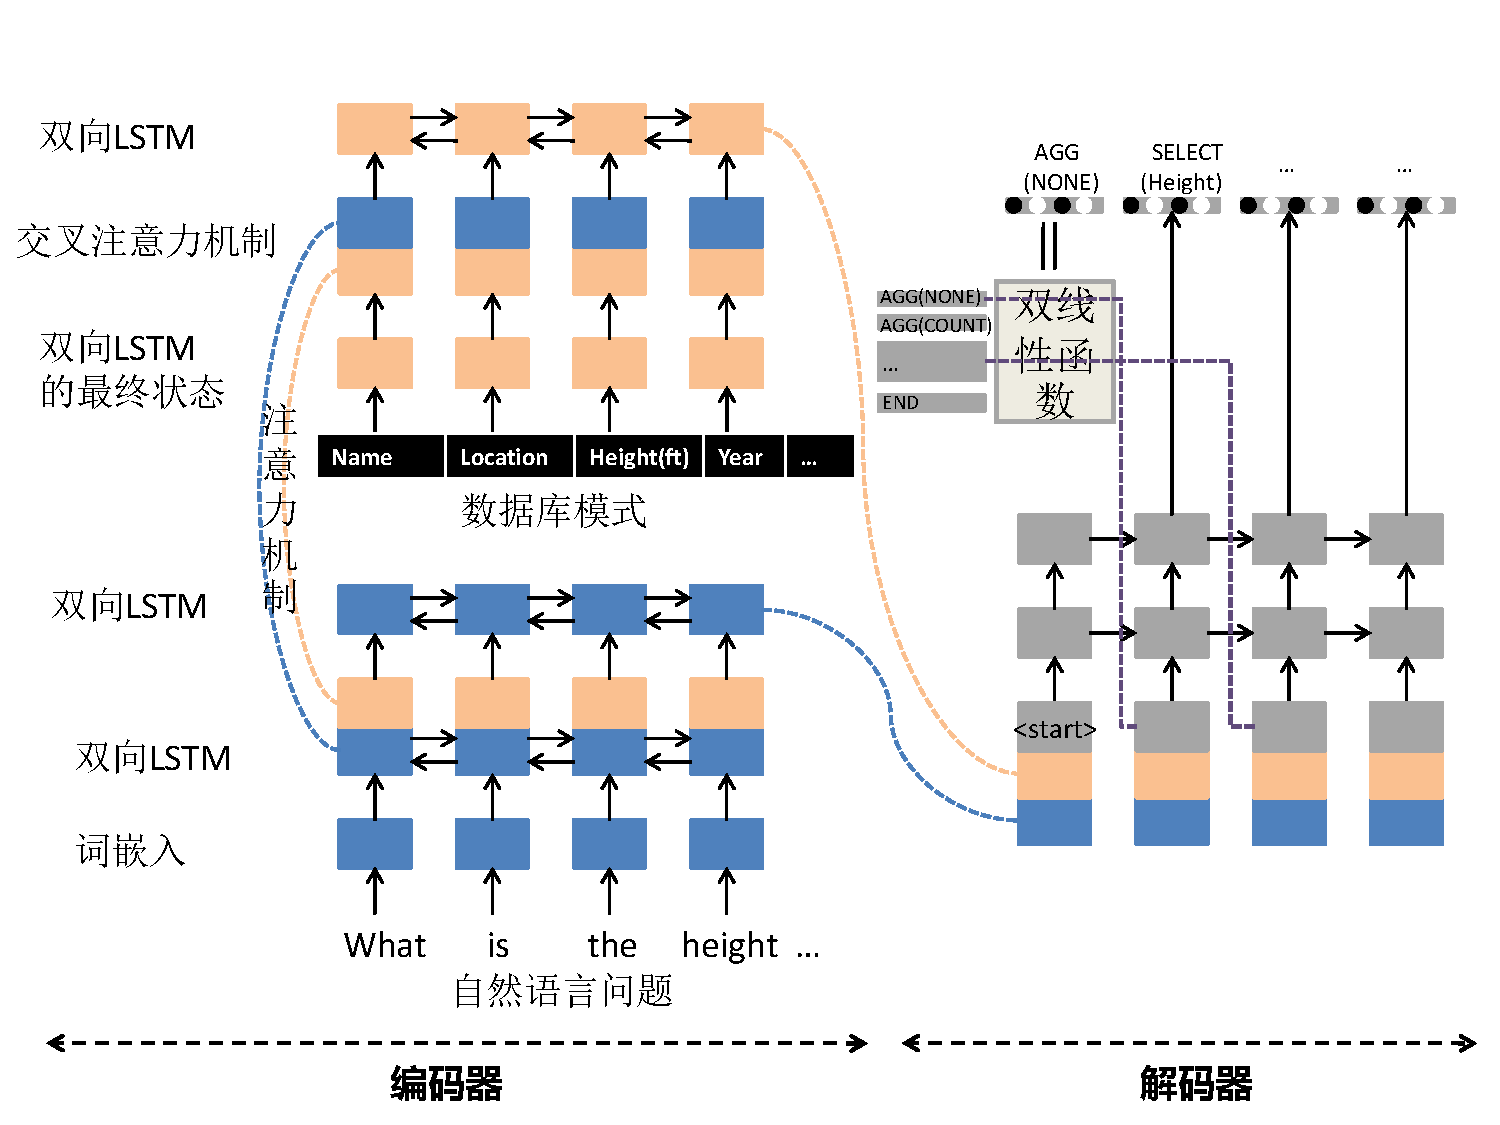
\includegraphics[width=15cm]{example/nl2sqlnet.pdf}
  \bicaption[基于深度强化学习的NL2SQL生成网络]
    {基于深度强化学习的NL2SQL生成网络}
    {The Network of NL2SQL With Deep Reinforcement Learning}
  \label{fig:nl2sqlnet}
\end{figure}


增强解析器的网络结构如图\ref{fig:nl2sqlnet}所示,包含编码器和解码器两个部分。
其中,编码器的具体步骤如下:
\begin{enumerate}
  \item 对于输入的句子$w$中的每个单词$w_i$,先将其使用词向量进行向量编码(word embedding)。
  \item 将其送入一个双向的长短期记忆网络(bi-directional Long Short-Term Memory,简称bi-LSTM),其中每个细胞(cell)会有一个隐状态$h^W_i$。
  \item 由于一个列名可能由一个或多个单词构成,我们对每个列名先进行词向量编码并输入一个bi-LSTM中,再使用从bi-LSTM中得到的最终的隐状态作为列名初始表示(initial representation)。
  \item 使用自注意力机制(self-attention\cite{vaswani2017attention})将该初始表示转换为$h^C_j$。
  \item 在得到$h^W_i$和$h^C_j$之后,使用缩放点积注意力\cite{vaswani2017attention}得到$h^C_j$和$h^W_i$的加权平均值并作为单词$w_i$和$c_j$的向量表示。
  \item 将这两个向量进行拼接并分别送入使用自然语言问题和列名作为输入的bi-LSTM中。这两个LSTM网络的隐状态就是我们所期望的向量表示$r^W_i$和$r^C_j$。
\end{enumerate}


\subsection{解码器}
\label{enl2sql:decoder}

在\ref{enl2sql:encoder}节中,我们已经获得了对于单词$w_i$的向量表示$r^W_i$和以及列名$c_j$的向量示$r^C_j$。
接下来是解码器部分的设计与细节。

首先,解码器的目标是为了对由输入$x$和历史动作$a_{<i}$构成的概率分布$P_{\theta}(a|x,a_{<i})$进行建模。其主要包括以下两点挑战:
\begin{enumerate}
  \item 动作(action)的不确定性:模型采取的动作都是取决于输入以及当前解析器的状态,而不是固定不变的。
  \item 增强解析器的决策完全依赖于其获得的上下文信息:增强解析器依赖于解码的历史信息以及输入的问题和列名信息。
\end{enumerate}

为了解决第一个问题,我们使用了基于LSTM的解码器架构并使用独立打分机制来对动作的可能性进行打分。
模型给每个候选的动作$a$打上分数$s_a$并且使用$softmax$函数将分数正则化(normalize)到一个概率分布上。
对于$i$时刻来说,我们用$h^{DEC}_i$来表示当前解码器的隐状态并且使用双线性函数$s_a = (h^{DEC}_i)^T U^A r^A_a$来给分数$a$建模。
双线性函数中$r^A_a$是由动作嵌入(action embedding)和参数表示(parameter representation)建模得到的动作$a$的向量表示。
其中参数表示已经在表\ref{enl2sql:dzqd}中给出。

我们使用点积注意力机制(dot-product attention)\cite{vaswani2017attention}来捕获模型决策与输入的问题和列名之间的依赖关系。
之后,将前一$i$时刻的输出动作表示$r^A_{a_i}$、自然语言问句的注意力向量$e^W_i$以及列名的注意力向量$e^C_i$拼接在一起,
作为$i+1$时刻的LSTM解码器的第一层的输入。
其中,向量$e^C_i = \sum_j \alpha_{i,j} r^C_j$,  $\alpha \propto h^{DEC}_i \cdot r^C_j$。
向量$e^W_i$的定义相似可得。



\subsection{过滤条件顺序问题和隐式列名问题}
\label{enl2sql:ndo}

在前文中,我们做出过一个假设,即每个自然语言问题都只会对应一条SQL查询语句,并且每个查询语句都只会对应一个正确的动作序列。
实际上,这个假设并不能完全成立。
一个简单的例子就是出现在WHERE子句里面的过滤条件的顺序并不确定,不同的过滤条件的顺序将会导致不同的动作序列。
除此之外,我们在\ref{enl2sql:icn}节中还介绍了另一个会产生歧义的情况,它会产生一个自然语言问题可以转换为多种SQL查询语句且其执行结果仍保持一致的问题。
对于最终用户而言,这些查询语句其实是完全等效的。

针对上述的两种情况,本文会将每个训练样本转换为多个序列以供参考并且在训练过程中使用多种目标策略。
参考语法分析领域的办法,本文会采用一个非确定的预言(oracle)从而使得解析器可以在多个动作序列中进行探索。
特别注意的是,在前文中所述的训练机制都是采用基于静态预言而非非确定预言的。

我们假定预言(oracle)$O$可在时刻$t$返回一组正确且连续的动作$O(x,a_{<t})$。
其中,将$O(x,a_{<t})$集合中的任何一个对象拿出来执行解析都可以得到最后的正确结果。
对于每一个训练样本$L_x$来说,其训练目标将被如公式\ref{enl2sql:eq3}定义。
\begin{equation}
  \label{enl2sql:eq3}
  L_x = \sum_{i=0}^k log \sum_{a\in O(x,a_{<i})} P_{\theta}(a|x,a_{<i})
\end{equation}
其中$a_{<i}$表示动作序列$a_{1},...,a_{i-1}$,
$a_{i} = \mathop{\arg\max}_{a\in O(x,a_{<i})}$,$a_i$代表在训练时解析器判定的置信度最高的动作。

当$O$是静态预言时,其只会包含一个单独且正确的动作,公式\ref{enl2sql:eq3}可被化简为一个简单的交叉熵的损失函数。
而当$O$是非确定的预言时,在训练期间,解析器会对多个不同的但是同样是正确的动作序列进行解析而不再是一个唯一的动作序列。

\subsubsection{解决过滤条件顺序问题}
\label{enl2sql:om}

训练一个形如text-to-SQL的解析器往往会碰到过滤条件顺序的问题。
在SQL查询语句中,过滤条件的先后顺序不会对语句的意图和执行结果产生影响。
但是在增强解析器模型中,我们需要将查询语句固定下来然后依据预定义的格式执行。
预测出的与训练集真值(groundtruth)的标签不同但是完全正确的语句可能没有办法得到适当的奖励(reward)。

有一些前人的研究使用了增强学习\cite{zhong2017seq2sql}或模块化的序列集成\cite{xu2017sqlnet}的方案来解决过滤条件顺序的问题。
其中,前者在一定程度上解决了这个问题但明显降低了模型的优化稳定性并导致训练时间大大增加。
而后者采用了一种较为复杂的模型设计来捕获子句之间的相互依赖关系,其预测出的过滤条件的信息将被用于预测下一个过滤条件。

在本章的方案中,本文利用一个非确定性的预言来解决过滤条件的顺序问题。
我们的模型结合了增量式方法的优势,利用子句之间的相互依赖性和模块化的方法来获得更高质量的训练信号。
具体来说,在预测下一个过滤条件的几个步骤中,模型会接受所有可能的后续条件(即尚未预测出的过滤条件)而忽视其位置所在。
对于图\ref{fig:nl2sqlexample}中给出的示例,除了本文在\ref{enl2sql:dzxl}节中给出的转换序列之外,
我们提出的非确定性的预言也接收$CONDCOL(c_2)$作为第二个动作的正确的延续。
如果模型即将预测出第一个动作,那么它将在预测第一个动作之前继续去预测第二个过滤条件是什么。
\subsubsection{解决隐式列名问题}
\label{enl2sql:icn}
在模型的初步验证实验过程中,我们观察到解析器模型在开发集上会产生一些错误的预测,其主要的出错原因是隐式列名的问题。
在很多场景下,自然语言的问题中并没有明确提到过滤条件中所需要的列名。
例如:在图\ref{fig:nl2sqlexample}中的问题中就没有直接提到“Name”这个列名。
同样地,“What is the area of Canada?”这个典型的自然语言问题中也没有出现关键词“country”。
对于我们人类而言,这种隐式的表达会使得我们的自然语言的问题更加简洁而且我们可以很快地从上下文的相关内容中轻易地推断出缺失的信息。
但是对于机器学习的模型来说,这些都会是巨大的挑战。

本文中,我们结合非确定性的预言及动作清单中的$ANYCOL$来解决隐式列名的问题。
在模型运行过程中,我们将根据过滤条件来拓展预测,从而模拟人类如何轻松找到未在问题中出现的列名的过程。
在图\ref{fig:nl2sqlexample}中的例子中,除了动作$CONDCOL(c_1)$外,我们还允许模型进行另一种的动作$CONDCOL(ANYCOL)$。
当$CONDCOL(ANYCOL)$出现时,例如此时的$ANYCOL='Willis Tower'$,我们会将它拓展为$Rank='Willis Tower' \quad OR \quad Name='Willis Tower' \quad OR \quad ...$。
这样一来,当列名没法被明确地解析出来时,非确定预言可以接收$ANYCOL$作为列名并且让我们的模型去预测哪种形式更容易被学习。


\section{实验与分析}
\subsection{数据集及评价指标}
WikiSQL是由Zhong\cite{zhong2017seq2sql}提出的第一个由自然语言问题、对应的SQL查询语句及数据表schema构成的大型数据集。
WikiSQL虽然在SQL语法上的覆盖范围比之前的数据集(例如,ATIS\cite{price1990evaluation,Dahl1994Expanding}和 GeoQuery\cite{Zelle2008Learning})要弱,
但是在问题、数据表模式和内容上具有很高的多样性。
这也使其在近期吸引了大量的研究人员的关注并使用神经网络进行建模和评估\cite{zhong2017seq2sql,dong2016language,xu2017sqlnet,yu2018typesql,wang2018pointing,huang2018natural,wang2018execution}。

在本章的实验中,我们采用了WikiSQL数据集中的默认划分,将数据集划分为训练集、验证集和测试集。
我们在验证集和测试集上对训练后的分别使用静态预言和非确定性预言的模型进行了评价。
在最后,我们会给出逻辑形式准确性(即SQL查询的精准匹配度)和执行准确性(即在数据库执行后可以产生相同的正确结果的比例),
其中执行准确性是我们优化的关键指标。


\subsection{实验设置}
在数据预处理过程中,我们大量借鉴了\cite{dong2018coarse}的方法对数据进行处理。
在词嵌入层(embedding layer)在训练集中出现至少两次的单词才会被保留在词汇表(vocabulary)中,剩下的将被赋予特殊的输入单元“UNK”。
我们使用已经训练好的Glove词嵌入\cite{pennington2014glove}并且可以在我们的模型训练时对词嵌入进行继续训练,该词嵌入的维度为16维。
我们还使用\cite{yu2018typesql}的方法对自然语言问题和列名进行了类型嵌入(type embedding):
对于每一个单词$w_i$和$c_j$,我们会判断其是否出现在列名中并给出一个离散的表示,而这些特征会被嵌入为4维的向量表示。
类型嵌入将会和词嵌入连接在一起并作为双向LSTM网络的输入。

另外,还需要说明的是,编码阶段的双向LSTM的单隐藏层的大小为256维,其中单向为128维。
解码阶段的LSTM由大小各为256的两个隐藏层组成。
所有的注意力连接都采用\ref{enl2sql:decoder}节中描述的点积形式。

在训练阶段,我们设置批尺寸(batch size)为64并使用0.3的丢失率(dropout rate)进行正则化处理。
同时,我们使用了ADAM优化器\cite{kingma2014adam}、设置初始学习率为默认值0.001用于参数的更新迭代以及将梯度修剪到5.0用于保证训练的稳定。


\subsection{实验结果}
\subsubsection{WIKISQL实验结果}

图\ref{fig:nl2sqlexample}为WikiSQL数据集\cite{zhong2017seq2sql}中的一个样例。
WikiSQL数据集是纯自然语言生成SQL查询语句的第一个数据集。
其中包含80654组自然语言问句及其对应的SQL查询语句,涵盖24241张从Wikipedia中获取的数据表。
从图中可以看到,NL2SQL任务的输入实际包括两部分:自然语言问题以及一个简单的数据表schema(schema代表数据表及表中的列)。

WikiSQL数据集中SQL查询语句具有一定的约束条件,必须符合如下模板:

\begin{table}[!hpb]
    \centering
    \bicaption[SQL查询语句模板]
      {SQL查询语句模板}
      {The Template of SQL Query Statement}
    \label{nli:sqlmb}
    \begin{tabular}{@{}llr@{}} \toprule
      % \multicolumn{2}{c}{Item} \\ \cmidrule(r){1-2}
    %   节点类型 & 对应的SQL组件\\\midrule
    \emph{SELECT   agg   selcol   WHERE   col   op   val   (AND   col   op   val)*}\\\bottomrule
  
      % Animal & Description & Price (\$)\\ \midrule
      % Gnat & per gram & 13.65 \\
      % & each & 0.01 \\
      % Gnu & stuffed & 92.50 \\
      % Emu & stuffed & 33.33 \\
      % Armadillo & frozen & 8.99 \\ \bottomrule
    \end{tabular}
  \end{table}

  在\ref{nli:sqlmb}中,\emph{selcol}代表表中的列名,\emph{agg}代表聚合操作(例如:COUNT,SUM或空),
  \emph{WHERE}后面为由一系列过滤调教构成的子句,每个\emph{op}代表一个过滤操作(例如:“=”),\emph{val}代表出现在自然语言问句中的过滤值。
  值得注意的是,尽管模板中的过滤条件服从标准的线性顺序,但由于存在\emph{AND}符号,所以过滤条件的先后顺序是无关紧要的。

\begin{table}[!htpb]
  \bicaption[WikiSQL中验证集和测试集的准确度]
    {WikiSQL中验证集和测试集的准确度}
    {The Accuracy Of Validation Sets And Test Sets In WikiSQL}
  \label{tab:wzyzjhcsjdzqd}
  \centering
  \begin{threeparttable}[b]
     \begin{tabular}{lcccc}
      \toprule
      \multirow{2}{10mm}{模型}&\multicolumn{2}{c}{验证集} & \multicolumn{2}{c}{测试集}\\
      \cmidrule(lr){2-3}\cmidrule(lr){4-5}
      % &www & \multicolumn{1}{c}{k} & www & k & www & k \\ % 使用说明符 d 的列会自动进入数学模式,使用 \multicolumn 对文字表头做特殊处理
      % TypeSQL引用 & Acc$_{lf}$ & Acc$_{ex}$ & Acc$_{lf}$ & Acc$_{ex}$\\
      & Acc$_{lf}$ & Acc$_{ex}$ & Acc$_{lf}$ & Acc$_{ex}$\\
      % TypeSQL引用 & 72.5 & 79.0 & 71.7 & 78.5\\
      \midrule
      TypeSQL模型(引用) & 72.5 & 79.0 & 71.7 & 78.5\\
      SQLNet模型(引用) & 76.1 & 82.0 & 75.4 & 81.4\\
      \midrule 
      本文提出的模型 &  &  &  & \\
      增强解析器(静态预言) & 76.1 & 82.5 & 75.5 & 81.6\\
      增强解析器(非确定性预言, 不解决过滤条件顺序问题) & 75.4 & 82.2 & 75.1 & 81.8\\
      % 增强解析器(非确定性预言, 解决过滤条件顺序问题) & 49.9 & 84.0 & 49.9 & 83.7\\
      % 增强解析器(非确定性预言, 解决过滤条件顺序问题) + EG (5) & 51.3 & 87.2 & 51.1 & 87.1\\
      增强解析器(非确定性预言) & 49.9 & 84.0 & 49.9 & 83.7\\
      增强解析器(非确定性预言) + EG (5) & 51.3 & 87.2 & 51.1 & 87.1\\
      % &$\underset{(2.12)}{4.22}$ & 120.0140\tnote{2} & 333.15 & 0.0411 & 444.99 & 0.1387 \\
      % &168.6123 & 10.86 & 255.37 & 0.0353 & 376.14 & 0.1058 \\
      % &6.761    & 0.007 & 235.37 & 0.0267 & 348.66 & 0.1010 \\
      \bottomrule
    \end{tabular}
    % \begin{tablenotes}
    % \item [1] the first note.% or \item [a]
    % \item [2] the second note.% or \item [b]
    % \end{tablenotes}
  \end{threeparttable}
\end{table}

实验的主要结果如表\ref{tab:wzyzjhcsjdzqd}所示。其中Acc$_{lf}$表示逻辑形式准确度,Acc$_{ex}$表示执行准确度,
“+ EG (5) ”表示使用执行引导策略且集束大小为5。

可以看到我们的增强解析器模型在使用静态预言的情况下就可以达到目前该领域的最高水平\cite{dong2018coarse}的范围。
在此基础之上,使用了非确定性预言的增强解析器在执行准确度上还可以大幅度提升2.1\%,但是其逻辑形式准确度反而会有所下降,
主要原因是使用了$ANYCOL$进行列的选择时,生成的SQL查询语句和真值(groundtruth)不能完全匹配。
我们还对过滤条件顺序问题和非确定性预言中的$ANYCOL$的贡献度进行了实验对比。
当我们的非确定性预言只用来解决\ref{enl2sql:om}节中的过滤条件顺序问题时,模型的性能和使用静态预言的模型大致相同。
我们认为这是因为在训练集中所出现的过滤条件的序列变化已经足够丰富,序列到动作的模型已经可以学习的很好。
除此之外,在预言中增加$ANYCOL$可以更好地捕捉到隐式的列明并提升性能,使得执行准确度从81.3\%增加至83.7\%。

我们的增强解析器模型在解码阶段使用的是贪心策略,即选择通过策略预测出的获得最高得分的动作。
同样,我们也可以使用集束搜索(beam search)来进行搜索。
其中,集束搜索是一种启发式的图搜索算法,为了减小搜索的空间与时间,在向图进行深度扩展时,去裁剪掉一些质量较差的节点,保留一些质量较高的节点。
使用集束搜索意味着我们可以在更大的搜索空间中进行搜索。
另外,我们还将执行引导策略和集束搜索策略结合在一起,进行执行引导的解码器可以避免生成语义错误的SQL查询语句,例如会产生运行时错误(runtime error)和空结果(empty result)错误的SQL查询语句。
除此之外有一点很关键,那就是将生成出的部分的输出放到数据库中的执行,得到的执行结果可以用来指导解码过程。
解码器可以维持一种部分输出的状态,该状态由聚合操作、选择列操作和完整的过滤条件构成。
在每个动作执行之后,由执行引导策略引导的解码器将保留前K个得分最高的且没有运行错误的SQL查询语句,在结束状态时从这K个语句中选择出最有可能的那个查询语句。
在K=5时,我们的模型在执行引导策略下载测试机上实现了87.1\%的执行准确度。

我们在表\ref{enl2sql:sybtjsdxdmxxn}中给出了具有执行引导过程的解码器在静态预言下的模型性能。
其中“+ EG ($k$)”的含义同表\ref{tab:wzyzjhcsjdzqd},k为集束大小。
其性能与非确定性预言下模型的性能非常接近,但需要更大的集束,也就意味着其解码的时间会大大增加。

\begin{table}[!hpb]
  \centering
  \bicaption[使用不同集束大小的模型性能]
    {使用不同集束大小的模型性能}
    {Model Performance With Different Beam Sizes}
  \label{enl2sql:sybtjsdxdmxxn}
  \begin{tabular}{ccccc} \toprule
    % \multicolumn{2}{c}{Item} \\ \cmidrule(r){1-2}
    \textbf{预言类型} & \textbf{w/o EG} & \textbf{+ EG (1)} & \textbf{+ EG (3)} & \textbf{+ EG (5)}\\\midrule
    静态 & 81.6 & 83.5 & 86.4 & 86.7\\
    非确定 & 83.7 & 86.0 & 87.1 & 87.1\\\midrule
    运行速度 (每秒运行的样本数) & 48.3 & 30.1 & 8.2 & 4.4\\
    \bottomrule
  \end{tabular}
\end{table}

\subsubsection{其他数据集实验结果}

除了在WikiSQL进行实验以为,本文还在ATIS\cite{Dahl1994Expanding}和Spider数据集\cite{yu2018spider}上进行了补充实验。

\textbf{ATIS数据集实验}

为了测试我们的模型是否可以推广到其他的数据集上,本文还是用了ATIS数据集进行了实验,数据在表\ref{tab:asjjsdsyjg}中给出。
ATIS数据集包含更多样的SQL结构,包括对多个表的查询以及嵌套查询。
为了和本文的任务设置相兼容,我们仅保留了ATIS数据集中没有嵌套查询的样本,即仅包含AND操作不包含INNER JOIN操作符。
我们会把多个相关的表进行JOIN连接并构造成单独的一个数据表以便我们的模型进行输入。
经过简化之后数据集共包含933个样本并分布在训练集、验证集和测试集中,并分别有714、93和126个样本。

\begin{table}[!htpb]
  \bicaption[ATIS数据集上的实验结果]
    {ATIS数据集上的实验结果}
    {The Experimental Results On The ATIS Dataset}
  \label{tab:asjjsdsyjg}
  \centering
  \begin{threeparttable}[b]
     \begin{tabular}{lcccc}
      \toprule
      \multirow{2}{10mm}{模型}&\multicolumn{2}{c}{验证集} & \multicolumn{2}{c}{测试集}\\
      \cmidrule(lr){2-3}\cmidrule(lr){4-5}
      % &www & \multicolumn{1}{c}{k} & www & k & www & k \\ % 使用说明符 d 的列会自动进入数学模式,使用 \multicolumn 对文字表头做特殊处理
      % TypeSQL引用 & Acc$_{lf}$ & Acc$_{ex}$ & Acc$_{lf}$ & Acc$_{ex}$\\
      & Acc$_{lf}$ & Acc$_{ex}$ & Acc$_{lf}$ & Acc$_{ex}$\\
      % TypeSQL引用 & 72.5 & 79.0 & 71.7 & 78.5\\
      \midrule
      增强解析器(静态预言) & 87.1 & 88.2 & 65.9 & 67.5\\
      增强解析器(非确定性预言, 不解决过滤条件顺序问题) & 88.1 & 89.2 & 68.3 & 69.1\\
      \bottomrule
    \end{tabular}
    % \begin{tablenotes}
    % \item [1] the first note.% or \item [a]
    % \item [2] the second note.% or \item [b]
    % \end{tablenotes}
  \end{threeparttable}
\end{table}

我们使用静态预言和不使用$ANYCOL$的非确定预言的模型进行训练,在测试集上分别达到了 67.5\%和69.1\%的准确性。
使用非确定预言的模型在性能上有大幅增强,这也验证了我们之前的假设:
与WikiSQL相比而言,ATIS是一个小得多的数据集,因此可以解决过滤条件顺序问题的模型的效果会有不小提升。
另外,需要说明的是,由于ATIS数据的性质,没有对$ANYCOL$进行测试。

\textbf{Spider数据集实验}

\begin{figure}[!htp]
  \centering
  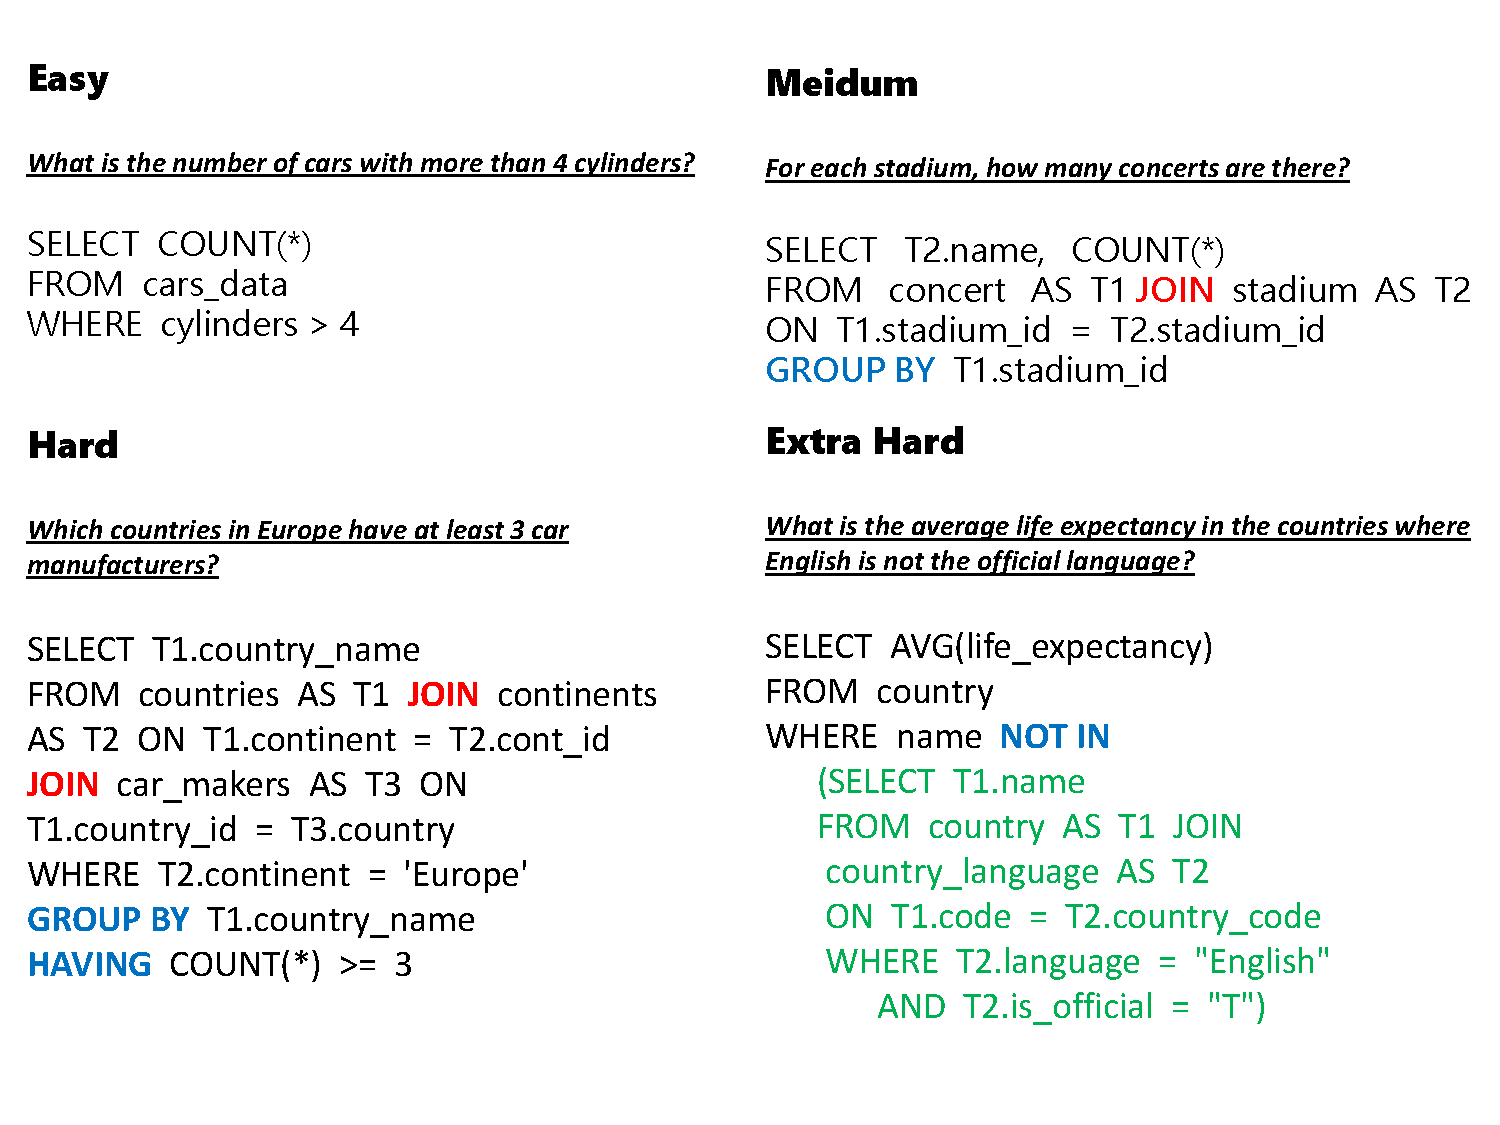
\includegraphics[width=15cm]{example/spider.pdf}
  \bicaption[Spider数据集样例]
    {Spider数据集样例}
    {Examples Of The Spider Dataset}
  \label{fig:spiderxample}
\end{figure}

spider数据集是一个由11名耶鲁大学学生标注的大型的跨域的包含语义解析和文本到SQL语句的数据集。
其挑战的目标为开发在跨域的数据集上开发自然语言接口。
spider数据集由200个数据库中的10181个问题和5693个SQL查询语句组成,并且其中有很多表覆盖了138个不同的域。
不同复杂程度的SQL查询会出现在训练集和测试集中,如图\ref{fig:spiderxample}中所示。
这也就要求模型需要具有较好的拓展性,从而适应新的SQL查询语句以及新的数据库模式。

\begin{figure}[!htp]
  \centering
  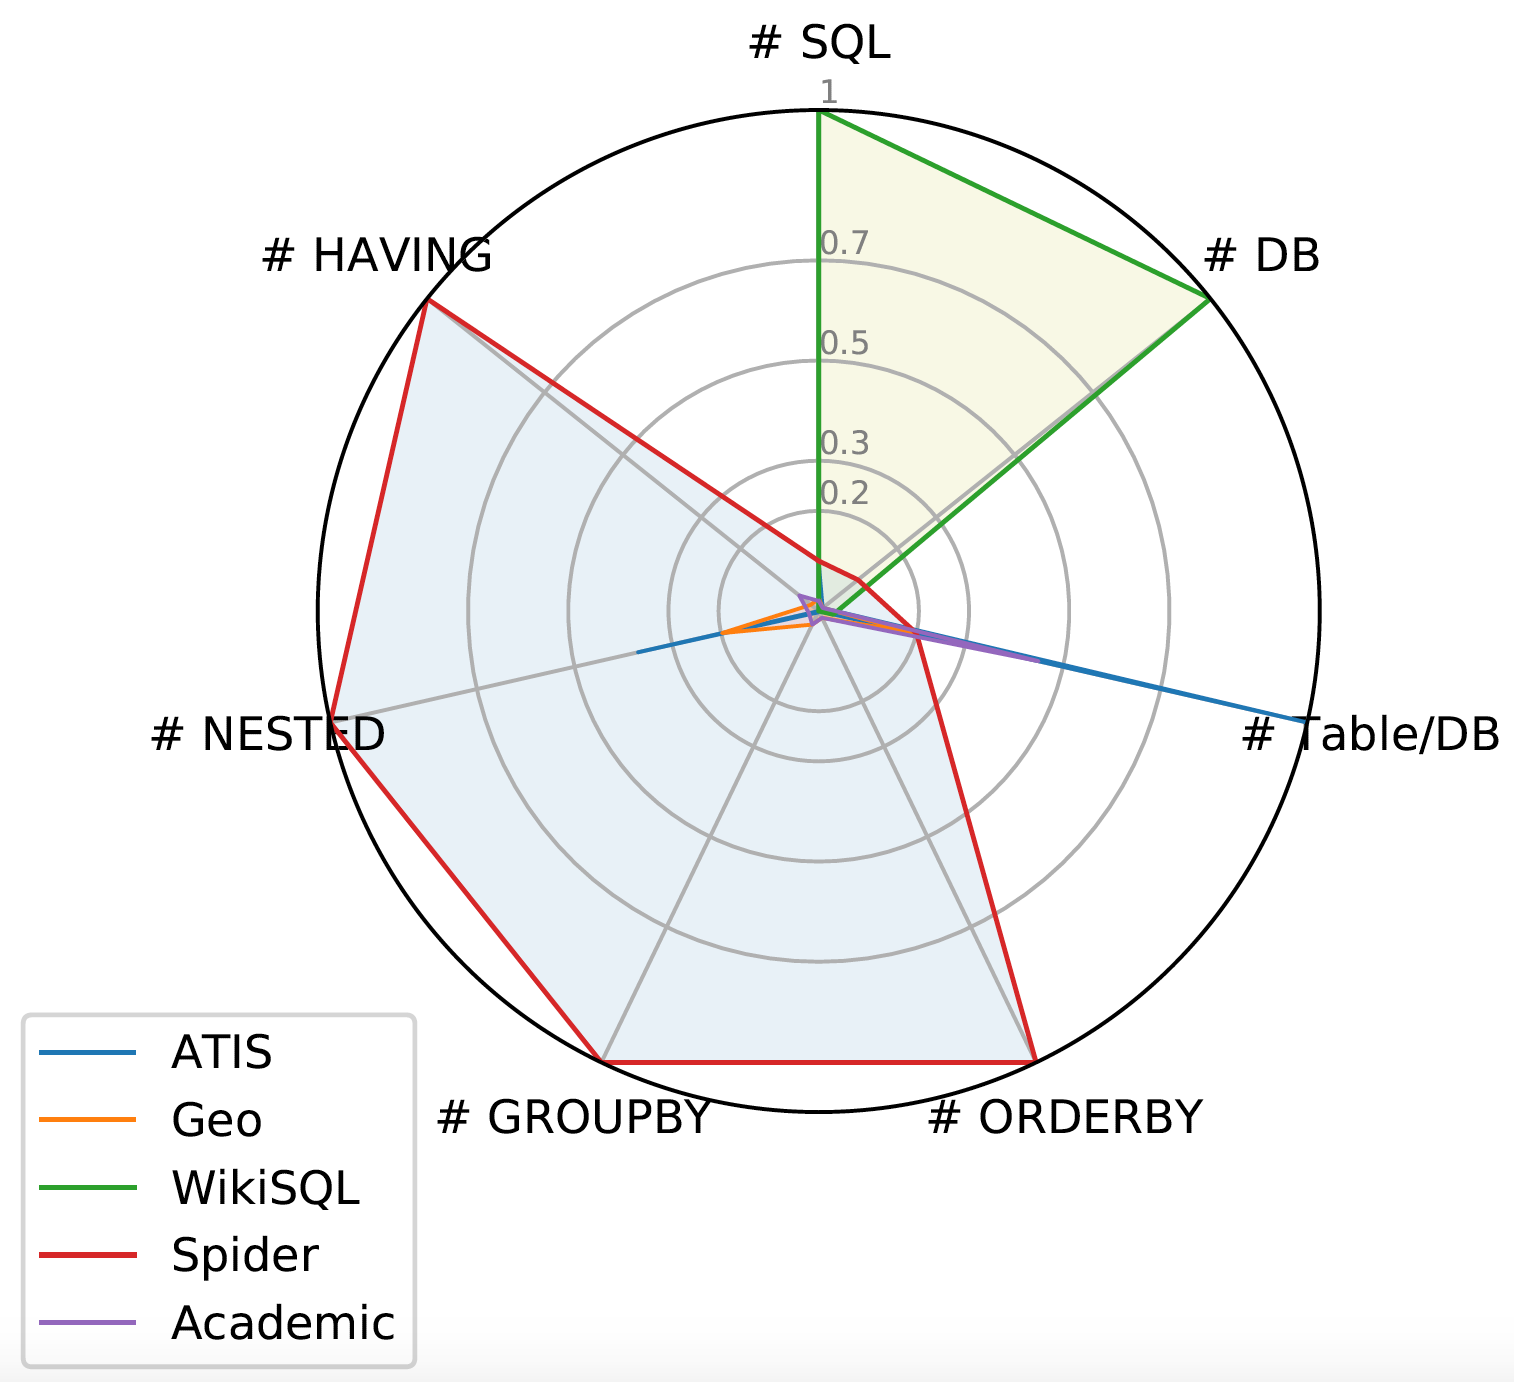
\includegraphics[width=10cm]{example/spiderchart.png}
  \bicaption[Spider数据集的组成]
    {Spider数据集的组成}
    {The Component of The Spider Dataset}
  \label{fig:spiderchart}
\end{figure}

如图\ref{fig:spiderchart}所示,spider数据集的1.0版本有别于其他之前的所有SQL语义解析的数据集:

\begin{itemize*}
  \item 对于ATIS, Geo和Academic数据集来说,每个数据集都只包含在一个数据库中执行的若干个SQL查询,并且SQL查询在训练集和测试集的分割时完全相同的。
  
  \item WikiSQL数据集中的SQL查询和表的数量都相对较大,但是所有的SQL查询语句都较为简单,并且每个数据库都只有一个没有任何外键的表。  
\end{itemize*}

所以,在spider数据集上的实验能够说明模型从简单的SQL查询语句生成到复杂的SQL查询语句生成的能力,说明模型的通用性与泛化性。

\begin{table}[!htpb]
  \bicaption[Spider数据集上的实验结果]
    {Spider数据集上的实验结果}
    {The Experimental Results On The Spider Dataset}
  \label{tab:ssjjsdsyjg}
  \centering
  \begin{threeparttable}[b]
     \begin{tabular}{lcc}
      \toprule
      模型 & 验证集 & 测试集\\
      % \cmidrule(lr){2-3}\cmidrule(lr){4-5}
      % &www & \multicolumn{1}{c}{k} & www & k & www & k \\ % 使用说明符 d 的列会自动进入数学模式,使用 \multicolumn 对文字表头做特殊处理
      % TypeSQL引用 & Acc$_{lf}$ & Acc$_{ex}$ & Acc$_{lf}$ & Acc$_{ex}$\\
      % & Acc$_{lf}$ & Acc$_{ex}$ & Acc$_{lf}$ & Acc$_{ex}$\\
      % TypeSQL引用 & 72.5 & 79.0 & 71.7 & 78.5\\
      \midrule
      Seq2Seq + attention & 1.8	& 4.8\\
      TypeSQL & 8.0	& 8.2\\
      SQLNet & 10.9	& 12.4\\
      SyntaxSQLNet & 18.9	& 19.7\\
      增强解析器(非确定性预言) + EG (5) & 23.2  & 24.1\\
      % 增强解析器(静态预言) & 87.1 & 88.2 & 65.9 & 67.5\\
      % 增强解析器(非确定性预言, 不解决过滤条件顺序问题) & 88.1 & 89.2 & 68.3 & 69.1\\
      \bottomrule
    \end{tabular}
    % \begin{tablenotes}
    % \item [1] the first note.% or \item [a]
    % \item [2] the second note.% or \item [b]
    % \end{tablenotes}
  \end{threeparttable}
\end{table}

从表\ref{tab:ssjjsdsyjg}可以看出,我们使用$ANYCOL$的非确定预言的模型进行测试,在测试集上分别达到了 23.2\%和24.1\%的准确性,超过了之前提出的所有方法。
使用非确定预言的模型可以很好地解决过滤条件顺序问题,所以在性能上表现优异。
同时,得益于$ANYCOL$机制对隐式列名问题的处理,在spider数据集上的表现证明了模型具有很好的泛化性能。


\section{本章小结}

本章提出了一种基于深度强化学习的NL2SQL生成的解决方案。
在离线训练阶段,将WikiSQL中的数据进行序列表示后输入给网络模型,模型生成SQL查询语句后在数据库中执行,再使用奖励函数构造奖励用于强化网络模型。
在在线生成阶段用户输入自然语言查询语句及数据库模式,训练好的网络模型将生成符合用户查询意图的SQL查询语句。
我们把其中最重要的网络模型称为“增强解析器”模型,它由编码器和解码器构成并结合了自注意力机制。
参考强化学习的基本范式,本章将增强解析器学习的目标转换为策略的优化问题并对解析器的状态和动作进行了定义。
为了解决SQL查询语句中的过滤条件的顺序问题以及隐式列名的问题,本章还提出了非确定性预言和$ANYCOL$状态的解决办法。
最后,本章与目前NL2SQL领域的前沿方法进行对比,在不同数据集上的实验结果证明了本文方法的有效性与前瞻性。